\documentclass[12pt]{beamer}
\usepackage{../Estilos/BeamerMAF}
\usepackage{../Estilos/ColoresLatex}
\usepackage[absolute, overlay]{textpos}

\usetheme{Copenhagen}
\usecolortheme{wolverine}
%\useoutertheme{default}
\setbeamercovered{invisible}
% or whatever (possibly just delete it)
\setbeamertemplate{section in toc}[sections numbered]
\setbeamertemplate{subsection in toc}[subsections numbered]
\setbeamertemplate{subsection in toc}{\leavevmode\leftskip=3.2em\rlap{\hskip-2em\inserttocsectionnumber.\inserttocsubsectionnumber}\inserttocsubsection\par}
% \setbeamercolor{section in toc}{fg=blue}
% \setbeamercolor{subsection in toc}{fg=blue}
% \setbeamercolor{frametitle}{fg=blue}
\setbeamertemplate{caption}[numbered]

\setbeamertemplate{footline}
\beamertemplatenavigationsymbolsempty
\setbeamertemplate{headline}{}


\makeatletter
% \setbeamercolor{section in foot}{bg=gray!30, fg=black!90!orange}
% \setbeamercolor{subsection in foot}{bg=blue!30}
% \setbeamercolor{date in foot}{bg=black}
\setbeamertemplate{footline}
{
  \leavevmode%
  \hbox{%
  \begin{beamercolorbox}[wd=.333333\paperwidth,ht=2.25ex,dp=1ex,center]{section in foot}%
    \usebeamerfont{section in foot} \insertsection
  \end{beamercolorbox}%
  \begin{beamercolorbox}[wd=.333333\paperwidth,ht=2.25ex,dp=1ex,center]{subsection in foot}%
    \usebeamerfont{subsection in foot}  \insertsubsection
  \end{beamercolorbox}%
  \begin{beamercolorbox}[wd=.333333\paperwidth,ht=2.25ex,dp=1ex,right]{date in head/foot}%
    \usebeamerfont{date in head/foot} \insertshortdate{} \hspace*{2em}
    \insertframenumber{} / \inserttotalframenumber \hspace*{2ex} 
  \end{beamercolorbox}}%
  \vskip0pt%
}
\makeatother

\makeatletter
\patchcmd{\beamer@sectionintoc}{\vskip1.5em}{\vskip0.8em}{}{}
\makeatother

% %\newlength{\depthofsumsign}
% \setlength{\depthofsumsign}{\depthof{$\sum$}}
% \newcommand{\nsum}[1][1.4]{% only for \displaystyle
%     \mathop{%
%         \raisebox
%             {-#1\depthofsumsign+1\depthofsumsign}
%             {\scalebox
%                 {#1}
%                 {$\displaystyle\sum$}%
%             }
%     }
% }
% \def\scaleint#1{\vcenter{\hbox{\scaleto[3ex]{\displaystyle\int}{#1}}}}
% \def\scaleoint#1{\vcenter{\hbox{\scaleto[3ex]{\displaystyle\oint}{#1}}}}
% \def\bs{\mkern-12mu}


\resetcounteronoverlays{saveenumi}

\AtBeginDocument{\RenewCommandCopy\qty\SI}
\ExplSyntaxOn
\msg_redirect_name:nnn { siunitx } { physics-pkg } { none }
\ExplSyntaxOff

\date{}

\title{\large{Funciones de Hermite}}
\subtitle{Tema 4 - Funciones Especiales}
\author{M. en C. Gustavo Contreras Mayén}

\resetcounteronoverlays{saveenumi}

\begin{document}
\maketitle
\fontsize{14}{14}\selectfont
\spanishdecimal{.}

\section*{Contenido}
\frame[allowframebreaks]{\frametitle{Contenido} \tableofcontents[currentsection, hideallsubsections]}

\section{El oscilador armónico cuántico}
\frame[allowframebreaks]{\frametitle{Contenido a revisar} \tableofcontents[currentsection, hideothersubsections]}
\subsection{Introducción}


%Referencia: Griffiths - Introduction to quantum mechanics. Cap. 2.3

\begin{frame}
\frametitle{El oscilador cuántico}
Sabemos que el oscilador armónico clásico consiste de una masa $m$ atada a un resorte con una constante $k$, el movimiento que describe la masa, sigue la ley de Hooke:
\pause
\begin{align*}
F = - k \, x = m \, \dv[2]{x}{t}
\end{align*}
\end{frame}
\begin{frame}
\frametitle{Solución directa}
Que tiene por solución (si omitimos la fricción):
\pause
\begin{align*}
x (t) = A \, \sin (\omega \, t) + B \, \cos (\omega \, t)
\end{align*}
\pause
donde:
\pause
\begin{equation}
\omega \equiv \sqrt{\dfrac{k}{m}}
\label{eq:ecuacion_02_036}
\end{equation}
es la frecuencia angular de oscilación.
\end{frame}
\begin{frame}
\frametitle{De la energía potencial}
La energía potencial correspondiente es:
\pause
\begin{equation}
V (x) = \dfrac{1}{2} k \, x^{2}
\label{eq:ecuacion_02_037}
\end{equation}
cuyo trazo es el de una parábola.
\end{frame}
\begin{frame}
\frametitle{¿Oscilador perfecto?}
De hecho, no existe como tal un oscilador armónico \textocolor{red}{perfecto}: \pause si estiramos demasiado el resorte, éste se romperá, por lo que la ley de Hooke ya no se cumple una vez que se alcanza este punto.
\end{frame}
\begin{frame}
\frametitle{Aproximación del potencial}
Podemos considerar que cualquier potencial es \textocolor{ao}{aproximadamente} parabólico en la vecindad de un mínimo local, como se puede ver en la figura (\ref{fig:figura_001}):
\end{frame}
\begin{frame}
\frametitle{Aproximación del potencial}
\begin{figure}[H]
    \centering
    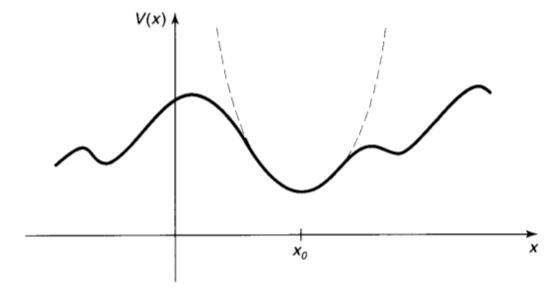
\includegraphics[scale=0.4]{Imagenes/Potencial_arbitrario.png}
    \caption{Aproximación parabólica (curva sesgada) en un potencial arbitrario, en la vecindad de un mínimo local.}
    \label{fig:figura_001}
\end{figure}
\end{frame}
\begin{frame}
\frametitle{Expandiendo el potencial}
Es posible expandir el potencial $V(x)$ es una serie de Taylor alrededor del mínimo:
\pause
\begin{align*}
V (x) &= V (x_{0}) {+} \pderivada{V} (x_{0}) (x {-} x_{0}) + \\[1em]
&+ \dfrac{1}{2} \sderivada{V} (x_{0}) (x {-} x_{0})^{2} + \ldots
\end{align*}
\end{frame}
\begin{frame}
\frametitle{Expandiendo el potencial}
Veamos que:
\pause
\setbeamercolor{item projected}{bg=aquamarine,fg=black}
\setbeamertemplate{enumerate items}{%
\usebeamercolor[bg]{item projected}%
\raisebox{1.5pt}{\colorbox{bg}{\color{fg}\footnotesize\insertenumlabel}}%
}
\begin{enumerate}[<+->]
\item Se puede eliminar $V(x_{0})$, ya que podemos agregar una constante al potencial $V(x)$ y no modifica en nada a la fuerza.
\item Tenemos que $\pderivada{V} (x_{0}) = 0$, ya que $x_{0}$ es un mínimo local.
\seti
\end{enumerate}
\end{frame}
\begin{frame}
\frametitle{Expandiendo el potencial}
\setbeamercolor{item projected}{bg=aquamarine,fg=black}
\setbeamertemplate{enumerate items}{%
\usebeamercolor[bg]{item projected}%
\raisebox{1.5pt}{\colorbox{bg}{\color{fg}\footnotesize\insertenumlabel}}%
}
\begin{enumerate}
\conti
\item Podemos descartar los términos de orden superior, que se anulan mientras $(x - x_{0})$ se mantenga pequeño.
\end{enumerate}
\end{frame}
\begin{frame}
\frametitle{Representando el potencial}
Por lo que el potencial se representa como:
\pause
\begin{align*}
V (x) \cong \dfrac{1}{2} \, \sderivada{V} (x_{0}) (x - x_{0})^{2}
\end{align*}
\pause
que describe un oscilación armónica (alrededor de $x_{0}$), con una constante efectiva del resorte:
\begin{align*}
k = \sderivada{V} (x_{0})
\end{align*}
\end{frame}
\begin{frame}
\frametitle{Consideración importante}
Considera que $\sderivada{V} (x_{0})\geq 0$, \pause tomando en cuenta de que $x_{0}$ es un mínimo local.
\\
\bigskip
\pause
En el extraño caso de que $\sderivada{V} (x_{0})= 0$, \pause la oscilación ya no se aproxima a la de un oscilador armónico.
\end{frame}
\begin{frame}
\frametitle{Relevancia del oscilador}
Esta es la importancia del oscilador armónico: \pause cualquier movimiento oscilatorio se puede aproximar a una oscilación armónica, mientras la amplitud sea pequeña.
\end{frame}

\section{El problema cuántico}
\frame[allowframebreaks]{\frametitle{Temas a revisar} \tableofcontents[currentsection, hideothersubsections]}
\subsection{Ecuación inicial}

\begin{frame}
\frametitle{Ecuación conocida}
El problema cuántico es resolver la ecuación de Schrödinger para el potencial:
\pause
\begin{equation}
V (x) = \dfrac{1}{2} m \, \omega^{2} \, x^{2}
\label{eq:ecuacion_02_038}
\end{equation}
\end{frame}
\begin{frame}
\frametitle{Ecuación sin dependencia temporal}
Por lo que la ecuación de Schrödinger independiente del tiempo es:
\pause
\begin{equation}
- \dfrac{\hbar}{2 m} \dv[2]{\psi}{x} + \dfrac{1}{2} m \, \omega \, x^{2} \, \psi = E \, \psi
\label{eq:ecuacion_02_039}
\end{equation}
\end{frame}
\begin{frame}
\frametitle{De cómo resolver la ecuación}
En la literatura se encontrarán dos enfoques completamente diferentes para resolver este problema:
\end{frame}
\begin{frame}
\frametitle{De cómo resolver la ecuación}
\setbeamercolor{item projected}{bg=bananayellow,fg=blue}
\setbeamertemplate{enumerate items}{%
\usebeamercolor[bg]{item projected}%
\raisebox{1.5pt}{\colorbox{bg}{\color{fg}\footnotesize\insertenumlabel}}%
}
\begin{enumerate}[<+->]
\item El primero es una solución de \textocolor{red}{fuerza bruta} directa a la ecuación diferencial, que utiliza el método de expansión en una serie de potencias: \pause tiene la virtud de que la misma estrategia se puede aplicar a muchos otros potenciales.
\seti
\end{enumerate}
\end{frame}
\begin{frame}
\frametitle{De cómo resolver la ecuación}
\setbeamercolor{item projected}{bg=bananayellow,fg=blue}
\setbeamertemplate{enumerate items}{%
\usebeamercolor[bg]{item projected}%
\raisebox{1.5pt}{\colorbox{bg}{\color{fg}\footnotesize\insertenumlabel}}%
}
\begin{enumerate}[<+->]
\conti
\item El segundo es una técnica algebraica \textocolor{armygreen}{diabólicamente inteligente}, que utiliza los llamados \textocolor{bole}{operadores de escalera}.
\end{enumerate}
\pause
Primero mostraremos el método algebraico, porque es más rápido y simple (y más divertido).
\end{frame}

\subsection{Método algebraico}

\begin{frame}
\frametitle{Reescribiendo la ecuación}
Antes de iniciar, vamos a escribir la ec. (\ref{eq:ecuacion_02_039}) de una manera más sugestiva:
\pause
\begin{equation}
\dfrac{1}{2 m} \left[ \left( \dfrac{\hbar}{i} \dv{x} \right)^{2} + (m \, \omega \, x)^{2} \right] \, \psi = E \, \psi
\label{eq:ecuacion_02_040}
\end{equation}
\pause
La idea es factorizar los términos dentro de los corchetes.
\end{frame}
\begin{frame}
\frametitle{Factorizando elementos}
Si éstos fueran números, podríamos hacerlo fácilmente, ya que:
\pause
\begin{align*}
u^{2} + v^{2} = (u - i \, v)(u + i \, v)
\end{align*}
Pero no del todo es simple, ya que $u$ y $v$ son \textocolor{byzantine}{operadores}, \pause y los operadores en general, \textocolor{blue-violet}{no conmutan} ($u \, v$ no es lo mismo que $v \, u$).
\end{frame}
\begin{frame}
\frametitle{Avanzando en el análisis}
Aún así, veamos la siguiente expresión:
\pause
\begin{equation}
a_{\pm} \equiv \dfrac{1}{\sqrt{2 m }} \left( \dfrac{\hbar}{i} \dv{x} \pm i \, m \, \omega \, x \right)
\label{eq:ecuacion_02_041}
\end{equation}
\pause
¿Cuál es el producto de $a_{-} \, a_{+}$? 
\end{frame}
\begin{frame}
\frametitle{Sobre el uso de los operadores}
\textocolor{red}{Advertencia}: \pause los operadores pueden ser complicados para trabajar en el concreto con ellos, \pause estamos obligados a cometer errores a menos que le asignemos una \enquote{función de prueba}, $f (x)$, para que actúen.
\end{frame}
\begin{frame}
\frametitle{Sobre el uso de los operadores}
Al final, podemos deshacernos de la función de prueba y quedaremos con una ecuación que involucra sólo a los operadores.
\end{frame}
\begin{frame}
\frametitle{Usando los operadores}
En nuestro caso del oscilador cuántico, tenemos:
\pause
\begin{eqnarray*}
\begin{aligned}
&a_{-} \, a_{+} \, f(x) =  \\[0.5em]
&\dfrac{1}{2 m} \left( \dfrac{\hbar}{i} \dv{x} - i \, m \, \omega \, x \right) \left( \dfrac{\hbar}{i} \dv{x} + i \, m \, \omega \, x \right) \, f(x) = \\[1em] \pause
&= \dfrac{1}{2 m} \left( \dfrac{\hbar}{i} \dv{x} - i \, m \, \omega \, x \right) \left( \dfrac{\hbar}{i} \dv{f}{x} + i \, m \, \omega \, x \, f \right) =
\end{aligned}
\end{eqnarray*}
\end{frame}
\begin{frame}
\frametitle{Usando los operadores}
\begin{eqnarray*}
\begin{aligned}
&= \dfrac{1}{2 m}  \left[ - \hbar^{2} \dv[2]{f}{x} + \hbar \, m \, \omega \dv{x} (x \, f) {-} \hbar \, m \, \omega \, x \, \dv{f}{x} + \right. \\[0.5em]
&+ \left. (m \, \omega \, x)^{2} \, f \right]  =\\[1em] \pause
&= \dfrac{1}{2 m} \left[ \left( \dfrac{\hbar}{i} \dv{x} \right)^{2} {+} (m \, \omega \, x)^{2} {+}\hbar \, m\, \omega \right] \, f(x)
\end{aligned}
\end{eqnarray*}
\end{frame}

\begin{frame}
\frametitle{Usando los operadores}
En el último paso hemos utilizado:
\pause
\begin{align*}
\dv{x} (x \, f) = x \left( \dv{f}{x} \right) + f
\end{align*}
\pause
Retirando la función de prueba, llegamos a que:
\pause
\begin{equation}
a_{-} \, a_{+} = \dfrac{1}{2 m} \left[ \left( \dfrac{\hbar}{i} \dv{x} \right)^{2} + (m \, \omega \, x)^{2} \right] + \dfrac{1}{2} \hbar \, \omega
\label{eq:ecuacion_02_042}
\end{equation}
\end{frame}
\begin{frame}
\frametitle{De la factorización}
Es claro que la ec. (\ref{eq:ecuacion_02_040}) no es factorizable de una manera perfecta, \pause ya que hay un término adicional: $(1/2) \hbar \, \omega$.
\end{frame}
\begin{frame}
\frametitle{De la factorización}
De todos modos, si ponemos este extra en el otro lado de la ecuación de Schrödinger, tenemos que:
\pause
\begin{equation}
(a_{-} \, a_{+} - \dfrac{1}{2} \hbar \, \omega) \, \psi = E \, \psi
\label{eq:ecuacion_02_43}
\end{equation}
\end{frame}
\begin{frame}
\frametitle{Orden de los factores}
Es importante considerar que el orden de los factores $a_{+}$ y $a_{-}$ es importante, con el mismo argumento con $a_{+}$ en la izquierda, llegamos a:
\pause
\begin{equation}
a_{+} \, a_{-} = \dfrac{1}{2 m} \left[ \left( \dfrac{\hbar}{i} \dv{x} \right)^{2} + (m \, \omega \, x)^{2} \right] - \dfrac{1}{2} \hbar \, \omega
\label{eq:ecuacion_02_044}
\end{equation}
\end{frame}
\begin{frame}
\frametitle{Orden de los factores}
Por lo tanto:
\pause
\begin{equation}
a_{-} \, a_{+} - a_{+} \, a_{-} = \hbar \, \omega
\label{eq:ecuacion_02_045}
\end{equation}
\end{frame}
\begin{frame}
\frametitle{La ecuación inicial}
La ecuación de Schrödinger se puede escribir como:
\pause
\begin{equation}
(a_{+} \, a_{-} + \dfrac{1}{2} \hbar \, \omega) \, \psi = E \, \psi
\label{eq:ecuacion_02_046}
\end{equation}
\end{frame}
\begin{frame}
\frametitle{Paso importante}
Ahora, aquí viene el paso crucial: \pause \textocolor{burgundy}{afirmamos que si $\psi$ cumple} con la ecuación de Schrödinger, con la energía $E$, \pause entonces $a_{+} \, \psi$ satisface la ecuación de Schrödinger con la energía $(E + \hbar \omega)$.
\end{frame}
\begin{frame}
\frametitle{Verificando el resultado}
Demostración:
\pause
\begin{eqnarray*}
\begin{aligned}
&(a_{+} \, a_{-} + \dfrac{1}{2} \hbar \, \omega) (a_{+} \, \psi) = \left( a_{+} \, a_{-} \, a_{+} + \dfrac{1}{2} \hbar \, \omega \, a_{+} \right) \psi = \\ \pause
&= a_{+} \left( a_{-} \, a_{+} + \dfrac{1}{2} \hbar \, \omega \right) \, \psi = \\ \pause
&= a_{+} \left[ \left( a_{-} \, a_{+} - \dfrac{1}{2} \hbar \, \omega \right) \, \psi + \hbar \, \omega \, \psi \right] \\ \pause
&= a_{+} (E \, \psi + \hbar \, \omega \, \psi) = \\ \pause
&= (E + \hbar \, \omega) (a_{+} \, \psi) \qed
\end{aligned}
\end{eqnarray*}
\end{frame}
\begin{frame}
\frametitle{Verificando el resultado}
Observemos que mientras que el orden de $a_{+}$ y de $a_{-}$ sí importa, \pause el ordenamiento de $a_{\pm}$ y cualquier constante (como $\hbar$, $\omega$, y $E$) no importa tanto.
\end{frame}
\begin{frame}
\frametitle{Verificando el resultado}
De la misma manera, $a_{-} \, \psi$ es una solución con energía $(E - \hbar \, \omega)$:
\pause
\begin{eqnarray*}
\begin{aligned}
&(a_{-} \, a_{+} - \dfrac{1}{2} \hbar \, \omega) (a_{-} \, \psi) = a_{-} \left( a_{+} \, a_{-} - \dfrac{1}{2} \hbar \, \omega \right) \, \psi = \\ \pause
&= a_{-} \left[ \left( a_{+} \, a_{-} + \dfrac{1}{2} \hbar \, \omega \right) \, \psi - \hbar \, \omega \, \psi \right] \\ \pause
&= a_{-} (E \, \psi - \hbar \, \omega \, \psi) = \\ \pause
&= (E - \hbar \, \omega) (a_{-} \, \psi) \qed
\end{aligned}
\end{eqnarray*}
\end{frame}
\begin{frame}
\frametitle{Lo que hemos obtenido}
Aquí, entonces, tenemos una máquina maravillosa para extraer nuevas soluciones, con energías más altas y más bajas, ¡si podemos encontrar una solución, para comenzar!
\end{frame}
\begin{frame}
\frametitle{Nombrando los operadores}
Llamamos a los $a_{\pm}$ \textocolor{cadmiumred}{operadores de escalera}, porque nos permiten subir y bajar en energía:
\pause
\setbeamercolor{item projected}{bg=carmine,fg=white}
\setbeamertemplate{enumerate items}{%
\usebeamercolor[bg]{item projected}%
\raisebox{1.5pt}{\colorbox{bg}{\color{fg}\footnotesize\insertenumlabel}}%
}
\begin{enumerate}[<+->]
\item $a_{+}$ se llama operador de subida (o de creación).
\item $a_{-}$ se llama operador de bajada (o de aniquilación) 
\end{enumerate}
\pause
La \enquote{escalera} de estados se ilustra en la figura (\ref{fig:figura_002}).
\end{frame}
\begin{frame}[plain]
\begin{figure}[H]
    \centering
    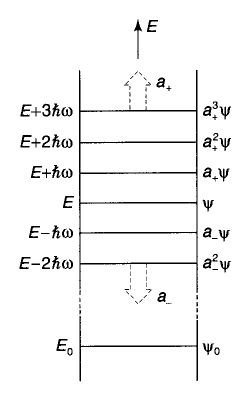
\includegraphics[scale=0.55]{Imagenes/Operadores_escalera.png}
    \caption{Escalera de estados estacionarios para el oscilador armónico.}
    \label{fig:figura_002}
\end{figure}
\end{frame}
\begin{frame}
\frametitle{¡Pero espera!}
¿Qué pasa si aplicamos el operador de bajada repetidamente? 
\\
\bigskip
\pause
¡Eventualmente llegaremos a un estado con una energía menor que cero, que no existe! \pause En algún momento la máquina debe fallar. \pause ¿Cómo puede suceder eso? 
\end{frame}
\begin{frame}
\frametitle{De la normalización}
Sabemos que $a_{-} \psi$ es una nueva solución para la ecuación de Schrödinger, \pause pero \textocolor{ceruleanblue}{no hay garantía de que sea normalizable}, \pause podría ser cero o su integral cuadrada podría ser infinita.
\end{frame}
\begin{frame}
\frametitle{Estado más bajo}
Conclusión: \pause Debe presentarse un \textocolor{coolblack}{peldaño más bajo} (llamémoslo $\psi_{0}$) tal que:
\pause
\begin{equation}
a_{-} \, \psi_{0} = 0
\label{eq:ecuacion_02_047}
\end{equation}
\end{frame}
\begin{frame}
\frametitle{Estado más bajo}
Es decir
\begin{align*}
\dfrac{1}{\sqrt{2 m}} \left( \dfrac{\hbar}{i} \, \dv{\psi_{0}}{x} - i \, m \, \omega \, x \, \psi_{0} \right) = 0
\end{align*}
\end{frame}
\begin{frame}
\frametitle{La ED a resolver}
La ED para $\psi_{0}$ es fácil de resolver:
\pause
\begin{eqnarray*}
\begin{aligned}
\scaleint{6ex} \dfrac{\dd{\psi_{0}}}{\psi_{0}} &= - \dfrac{m \, \omega}{\hbar} \scaleint{6ex} x \dd{x} \\[0.5em] \pause
\Longrightarrow \hspace{0.5cm} &\ln \psi_{0} = - \dfrac{m \, \omega}{2 \, \hbar} \, x^{2} + \text{ constante}
\end{aligned}
\end{eqnarray*}
\end{frame}
\begin{frame}
\frametitle{La ED a resolver}
Entonces:
\pause
\begin{equation}
\psi_{0} (x) = A_{0} \, \exp \left( - \dfrac{m \, \omega}{2 \, \hbar} x^{2} \right)
\label{eq:ecuacion_02_048}
\end{equation}
\pause
Calculemos el valor de $A$.
\end{frame}
\begin{frame}
\frametitle{El coeficiente}
Al normalizar, se tiene que:
\begin{eqnarray*}
\begin{aligned}
1 &= \abs{A}^{2} \scaleint{6ex}_{\bs - \infty}^{\infty} \exp \left( - \dfrac{m \, \omega \, x^{2}}{\hbar} \right) \dd{x} = \\[0.5em] \pause
&= \abs{A}^{2} \, \sqrt{\dfrac{\pi \hbar}{m \omega}}
\end{aligned}
\end{eqnarray*}
\end{frame}
\begin{frame}
\frametitle{El coeficiente}
Por lo que la solución es:
\pause
\begin{align*}
\psi_{0} (x) = \left( \dfrac{m \omega}{\pi \hbar} \right)^{\frac{1}{4}} \, \exp \left( - \dfrac{m \, \omega}{2 \, \hbar} x^{2} \right)
\end{align*}
\end{frame}
\begin{frame}
\frametitle{El nivel de energía}
Para conocer la energía en este estado, usamos este resultado en la ecuación de Schrödinger -en la forma de la ec. (\ref{eq:ecuacion_02_046})-
\begin{align*}
a_{+} \, a_{-} + (1/2) \hbar \omega = E_{0} \, \psi_{0}
\end{align*}
y aprovechamos el hecho de que $a_{-} \, \psi_{0} = 0$.
\end{frame}
\begin{frame}
\frametitle{El nivel de energía}
Por lo que:
\pause
\begin{equation}
E_{0} = \dfrac{1}{2} \hbar \, \omega
\label{eq:ecuacion_02_049}
\end{equation}
\pause
Ahora con nuestro pie firmemente plantado en el \textocolor{cornellred}{peldaño inferior}: \pause el estado fundamental del oscilador cuántico, o de energía cero.
\end{frame}
\begin{frame}
\frametitle{Consideración}
Toma en cuenta que solo puede haber una escalera, ya que el estado más bajo está determinado únicamente por la ec. (\ref{eq:ecuacion_02_047}).
\\
\bigskip
\pause
Para recuperar otros estados, simplemente aplicamos el operador de subida para generar los estados excitados.
\end{frame}
\begin{frame}
\frametitle{Consideración}
En el caso del oscilador armónico, es conveniente apartarse de la costumbre habitual y numerar los estados que comienzan con $n = 0$ en lugar de $n = 1$.
\end{frame}
\begin{frame}
\frametitle{Las soluciones obtenidas}
Así, de hecho, se han obtenido todas las soluciones (normalizables):
\pause
\begin{eqnarray}
\begin{aligned}
\psi_{n} (x) &= A_{n} \, (a_{+})^{n} \, \psi_{0} \\[0.5em]\pause
E_{n} &= \left( n + \dfrac{1}{2} \right) \hbar \, \omega
\end{aligned}
\label{eq:ecuacion_02_050}
\end{eqnarray}
\pause
Este método no determina de manera automática la normalización del factor $A_{n}$.
\end{frame}
\begin{frame}
\frametitle{Un estado de la solución}
Por ejemplo:
\begin{eqnarray*}
\begin{aligned}
\psi_{1} &= A_{1} \, a_{+} \, \psi_{0} = \\[1em] \pause
&= A_{1} \, \dfrac{1}{\sqrt{2 m}} \left( \dfrac{\hbar}{i} \, \dv{x} + i \, m \, \omega \, x \right) \, \exp \left( - \dfrac{m \, \omega}{2 \, \hbar} x^{2} \right) = \\[1em] \pause
&= \dfrac{A_{1}}{\sqrt{2 m}} \left[ \dfrac{\hbar}{i} \, \left( - \dfrac{m \, \omega}{\hbar} x \right)  \, \exp \left( - \dfrac{m \, \omega}{2 \, \hbar} x^{2} \right) +  \right.\\[0.5em]
&+ \left. i \, m \, \omega \, x \, \exp \left( - \dfrac{m \, \omega}{2 \, \hbar} x^{2} \right) \right] 
\end{aligned}
\end{eqnarray*}
\end{frame}
\begin{frame}
\frametitle{Un estado de la solución}
Que se simplifica como:
\pause
\begin{equation}
\psi_{1} (x) = \left( i \, A_{1} \, \omega \, \sqrt{2 m }  \right) \, x \, \exp \left( - \dfrac{m \, \omega}{2 \, \hbar} x^{2} \right)
\label{eq:ecuacion_02_051}
\end{equation}
\end{frame}
\begin{frame}
\frametitle{Calculando $A_{1}$}
Para calcular el valor de $A_{1}$, se tiene que:
\begin{eqnarray*}
\begin{aligned}
\psi_{1} = A_{1} \left( \dfrac{m \omega}{\pi \hbar} \right)^{\frac{1}{4}} \, \sqrt{\dfrac{2 m \omega}{\hbar}}
 x \, \exp \left( - \dfrac{m \omega}{2 \hbar} x^{2} \right) = \\ \pause
 \end{aligned}
\end{eqnarray*}
\end{frame}
\begin{frame}
\frametitle{Normalizando}
Al normalizar la función de onda:
\pause
\begin{eqnarray*}
\begin{aligned}
&\scaleint{6ex} \abs{\psi_{1}}^{2} \dd{x} = \\ \pause
&\abs{A_{1}}^{2} \sqrt{\dfrac{m \omega}{\pi \hbar}} \left( \dfrac{2 m \omega}{\hbar} \right) \scaleint{6ex}_{\bs -\infty}^{\infty} x^{2} \exp\left( - \dfrac{m \omega}{\hbar} x^{2} \right) \dd{x} = \\ \pause
&= \abs{A_{1}}^{2}
\end{aligned}
\end{eqnarray*}

\end{frame}
\begin{frame}
\frametitle{Resultado}
Se tiene entonces que:
\pause
\begin{align*}
\abs{A_{1}}^{2} = 1
\end{align*}
\end{frame}
\begin{frame}
\frametitle{Para otros estados}
No quisiéramos calcular $\psi_{50}$ de esta manera, \pause pero no importa: hemos encontrado todas las energías permitidas y en principio, hemos determinado los estados estacionarios, el resto es solo cálculo.
\end{frame}

% \textbf{Problemas a cuenta:}
% \begin{enumerate}
% \item Los operadores de subida y bajada generan nuevas soluciones a la ecuación de Schrödinger, pero éstas nuevas soluciones no están correctamente normalizadas. Por lo tanto, $a_{+} \, \psi_{n}$ es proporcional a $\psi_{n+1}$, y $a_{-} \,\psi_{n}$ es proporcional a $\psi_{n+1}$, pero nos gustaría conocer de manera precisa las constantes de proporcionalidad. Usando la integración por partes y la ecuación de Schrödinger (ecs. (\ref{eq:ecuacion_02_43}) y (\ref{eq:ecuacion_02_046})) para mostrar que
% \begin{align*}
% \scaleint{6ex}_{-\infty}^{\infty} \abs{a_{+} \, \psi_{n}}^{2} \dd{x} &= (n + 1) \hbar \, \omega \\
% \scaleint{6ex}_{-\infty}^{\infty} \abs{a_{-} \, \psi_{n}}^{2} \dd{x} &= n \, \hbar \, \omega
% \end{align*}
% y por tanto
% \begin{align}
% a_{+} \, \psi_{n} &= i \, \sqrt{(n + 1) \hbar \, \omega} \, \psi_{n+1} \label{eq:ecuacion_02_052} \\
% a_{-} \, \psi_{n} &= - i \, \sqrt{n \, \hbar \, \omega} \, \psi_{n-1} \label{eq:ecuacion_02_053}
% \end{align}
% \item Usando la ec. (\ref{eq:ecuacion_02_052}) demuestra que la constante de normalización $A_{n}$ en la ec. (\ref{eq:ecuacion_02_050}) es
% \begin{equation}
% A_{n} = \left( \dfrac{m \, \omega}{\pi \, \hbar} \right)^{1/4} \, \dfrac{(-i)^{n}}{\sqrt{n! (\hbar \, \omega)^{n}}}
% \label{eq:ecuacion_02_054}
% \end{equation}
% \end{enumerate}

\subsection{Método analítico}

\begin{frame}
\frametitle{De nuevo con la ED inicial}
Regresamos nuevamente a la ecuación de Schrödinger para el oscilador armónico (ec. \ref{eq:ecuacion_02_039}):
\pause
\begin{align*}
- \dfrac{\hbar}{2 m} \dv[2]{\psi}{x} + \dfrac{1}{2} m \, \omega \, x^{2} \, \psi = E \, \psi  
\end{align*}
\end{frame}
\begin{frame}
\frametitle{Ajustando la expresión}
Para un desarrollo más claro, hacemos el siguiente cambio de variable adimensional:
\pause
\begin{equation}
\xi \equiv \sqrt{ \dfrac{m \omega}{\hbar}} \, x
\label{eq:ecuacion_02_055}
\end{equation}
\end{frame}
\begin{frame}
\frametitle{La ED reescrita}
Por lo que en términos de $\xi$, la ecuación de Schrödinger toma la forma:
\pause
\begin{equation}
\dv[2]{\psi}{\xi} = (\xi^{2} - K) \, \psi
\label{eq:ecuacion_02_056}
\end{equation}
donde $K$ es la energía, en unidades de $(1/2) \hbar \omega$:
\pause
\begin{equation}
K = \equiv \dfrac{2 \, E}{\hbar \, \omega}
\label{eq:ecuacion_02_057}
\end{equation}
\end{frame}
\begin{frame}
\frametitle{Problema a resolver}
Nuestro problema es resolver la ec. (\ref{eq:ecuacion_02_056}), y durante el proceso obtener los valores \textocolor{darkblue}{permitidos} de $K$ (y por tanto de $E$).
\end{frame}
\begin{frame}
\frametitle{Revisando los valores}
Para iniciar, veamos que para valores muy grandes de $\xi$ (que a la vez, es decir que tendríamos valores muy grandes de $x$), \pause el término $\xi^{2}$ domina sobre la constante $K$, por lo que tendríamos:
\pause
\begin{equation}
\dv[2]{\psi}{\xi} \approx \xi^{2} \, \psi
\label{eq:ecuacion_02_058}
\end{equation}
\end{frame}
\begin{frame}
\frametitle{Solución a la ED}
Que tiene por solución:
\pause
\begin{equation}
\psi (\xi) \approx A \, \exp \left( - \dfrac{\xi^{2}}{2} \right) + B \, \exp \left( + \dfrac{\xi^{2}}{2} \right)
\label{eq:ecuacion_02_059}
\end{equation}
\pause
en donde encontramos que el término $B$ no se puede normalizar (no funciona cuando $\abs{x} \to \infty$).
\end{frame}
\begin{frame}
\frametitle{Soluciones aceptables}
Por lo que las soluciones aceptables con sentido físico, tienen las forma asintótica:
\pause
\begin{equation}
\psi (\xi) = ( \quad ) \exp \left( - \dfrac{\xi^{2}}{2} \right) 
\label{eq:ecuacion_02_060}
\end{equation}
con valores grandes de $\xi$.
\end{frame}
\begin{frame}
\frametitle{Influencia del término exponencial}
Esto sugiere que \enquote{aprovechamos} la parte exponencial:
\pause
\begin{equation}
\psi (\xi) = h (\xi) \, \exp \left( - \dfrac{\xi^{2}}{2} \right)
\label{eq:ecuacion_02_061}
\end{equation}
\pause
esperando que lo que queda de $[h (\xi)]$ tenga una forma funcional más simple que $\psi (\xi)$ mismo.
\end{frame}
\begin{frame}
\frametitle{Otra consideración}
Toma en cuenta que aunque invocamos algunas aproximaciones para motivar la ec. (\ref{eq:ecuacion_02_061}), lo que sigue es exacto. 
\\
\bigskip
\pause
La técnica para eliminar el comportamiento asintótico es el primer paso estándar en el método de la serie de potencias para resolver ecuaciones diferenciales.
\end{frame}
\begin{frame}
\frametitle{Manejando la expresión}
Diferenciando la ec. (\ref{eq:ecuacion_02_061}), se tiene que:
\pause
\begin{align*}
\dv{\psi}{\xi} = \left( \dv{h}{\xi} - \xi \, h \right) \, \exp \left( - \dfrac{\xi^{2}}{2} \right)
\end{align*}
\pause
por lo que la ec. de Schrödinger (ec. \ref{eq:ecuacion_02_056}) es:
\pause
\begin{equation}
\dv[2]{h}{\xi} - 2 \, \xi \, \dv{h}{\xi} +  (K - 1) \, h = 0
\label{eq:ecuacion_02_062}
\end{equation}
\end{frame}
\begin{frame}
\frametitle{Solución de propuesta}
Proponemos una solución a la ED (\ref{eq:ecuacion_02_062}) en la forma de una serie de potencias en $\xi$:
\pause
\begin{equation}
h (\xi) = a_{0} + a_{1} \, \xi + a_{2} \, \xi^{2} + \ldots = \nsum_{j=0}^{\infty} a_{j} \, \xi^{j}
\label{eq:ecuacion_02_063}
\end{equation}
\end{frame}
\begin{frame}
\frametitle{Diferenciando la solución}
Diferenciamos en dos ocasiones la solución para obtener:
\pause
\begin{eqnarray*}
\begin{aligned}
\dv{h}{\xi} &= \nsum_{j=0}^{\infty} j \, a_{j} \, \xi^{j-1} \\[0.5em] \pause
\dv[2]{h}{\xi} &= \nsum_{j=0}^{\infty} (j + 1)(j + 2) \, a_{j+2} \, \xi^{j}
\end{aligned}
\end{eqnarray*}
\end{frame}
\begin{frame}
\frametitle{Manejando la expresión}
Que al sustituir en la ec. (\ref{eq:ecuacion_02_062}), tenemos que:
\pause
\begin{equation}
\nsum_{j=0}^{\infty} \big[ (j {+} 1)(j {+} 2) \, a_{j+2} {-} 2 \, j \, a_{j} +  (K {-} 1) \, a_{j} \big] \, \xi^{j} = 0
\label{eq:ecuacion_02_64}
\end{equation}
\pause
Sabemos que los coeficientes para cada potencia de $\xi$ deben de anularse:
\end{frame}
\begin{frame}
\frametitle{Manejando la expresión}
Por tanto:
\pause
\begin{align*}
(j + 1)(j + 2) \, a_{j+2} - 2 \, j \, a_{j} +  (K - 1) \, a_{j} = 0
\end{align*}
\pause
de donde se obtiene que:
\pause
\begin{equation}
a_{j+2} = \dfrac{(2 \, j + 1 - K)}{(j + 1)(j + 2)} \, a_{j}
\label{eq:ecuacion_02_065}
\end{equation}
\pause
Esta es la \textocolor{blue}{regla de recursividad}, que es, en sí misma, equivalente a la ecuación de Schrödinger.
\end{frame}
\begin{frame}
\frametitle{Obteniendo los coeficientes}
Dado $a_{0}$, podemos obtener $a_{2}, a_{4}, a_{6}, \ldots$, \pause también para un $a_{1}$ dado, podemos obtener los $a_{3}, a_{5}, a_{7}, \ldots$
\end{frame}
\begin{frame}
\frametitle{Escribiendo un término}
Podemos escribir:
\pause
\begin{equation}
h (\xi) = h_{\text{par}} (\xi) + h_{\text{impar}} (\xi)
\label{eq:ecuacion_02_066}
\end{equation}
\pause
donde:
\pause
\begin{align*}
h_{\text{par}} (\xi) = a_{0} + a_{2} \, \xi^{2} + a_{4} \, \xi^{4} + \ldots
\end{align*}
Si es una función par de $\xi$ (ya que involucra sólo potencias pares) a partir de $a_{0}$.
\end{frame}
\begin{frame}
\frametitle{Paridad de la función}
Y como:
\pause
\begin{align*}
h_{\text{impar}} (\xi) = a_{1} \, \xi + a_{3} \, \xi^{3} + a_{5} \, \xi^{5} + \ldots
\end{align*}
si es función impar, a partir de $a_{1}$.
\end{frame}
\begin{frame}
\frametitle{Estableciendo la función}
Entonces tenemos que la ec. (\ref{eq:ecuacion_02_065}) determina a $h(\xi)$ en términos de dos constantes arbitrarias ($a_{0}$ y $a_{1}$), que es lo que se esperaba, dado que tenemos una ED2.
\end{frame}
\begin{frame}
\frametitle{Estableciendo la función}
Aún así, no todas las soluciones que se obtienen son normalizables.
\\
\bigskip
\pause
Para valores grandes de $j$, la fórmula de recursión pasa a ser (aproximadamente):
\pause
\begin{align*}
a_{j+2} \approx \dfrac{2}{j} \, a_{j}
\end{align*}
\end{frame}
\begin{frame}
\frametitle{Solución aproximada}
Con una solución (aproximada):
\pause
\begin{align*}
a_{j} \approx \dfrac{C}{(j/2)!}
\end{align*}
\pause
para alguna constante $C$.
\end{frame}
\begin{frame}
\frametitle{Para otros valores}
Esto nos lleva a (para valores grandes de $\xi$, donde las potencias elevadas dominan):
\pause
\begin{eqnarray*}
\begin{aligned}
h (\xi) &\approx C \nsum \dfrac{1}{(j/2)!} \, \xi^{j} \\[0.5em] \pause
&\approx C \nsum \dfrac{1}{k!} \xi^{2 k} \\[0.5em] \pause
&\approx C \, \exp \left( \xi^{2} \right)
\end{aligned}
\end{eqnarray*}
\end{frame}
\begin{frame}
\frametitle{Comportamiento no deseable}
Veamos ahora lo siguiente: si $h \to \exp \left( \xi^{2} \right)$.
\\
\bigskip
\pause
Entonces ¿$\psi \to \exp \left( \xi^{2}/2 \right)$?:
\\
\bigskip
\pause
!NO, ya que se presenta un comportamiento asintótico que no se desea!
\end{frame}
\begin{frame}
\frametitle{Corrigiendo la solución}
Solo hay una forma de salir de esto: \pause para soluciones normalizables, \textocolor{red}{la serie de potencias debe terminar}. 
\end{frame}
\begin{frame}
\frametitle{Corrigiendo la solución}
Debe de presentarse un valor \textocolor{carmine}{mayor} de $j$ (llámase $n$) \pause de manera que la fórmula de recursión devuelva un $a_{n+2} = 0$ 
\\
\bigskip
\pause
Esto truncará cada una de las series par o impar; la otra debe ser cero desde el principio.
\end{frame}
\begin{frame}
\frametitle{Soluciones congruentes}
Para soluciones físicamente aceptables, entonces, debemos tener que:
\pause
\begin{align*}
K = 2 \, n + 1
\end{align*}
para un entero positivo $n$
\end{frame}
\begin{frame}
\frametitle{Valor de la energía}
Es decir (refiriéndose a la ecuación (\ref{eq:ecuacion_02_057})) que la energía debe ser de la forma:
\pause
\begin{equation}
E_{n} = \left( n + \dfrac{1}{2} \right) \, \hbar \, \omega , \hspace{1.5cm} n = 0, 1, 2, \ldots
\label{eq:ecuacion_02_067}
\end{equation}
\end{frame}
\begin{frame}
\frametitle{Resultado interesante}
Así recuperamos, mediante un método completamente diferente, \pause la condición fundamental de \textocolor{cobalt}{cuantificación} que encontramos algebraicamente en la ec. (\ref{eq:ecuacion_02_050}).
\end{frame}
\begin{frame}
\frametitle{Valores permitidos}
Para los valores permitidos de $K$, la fórmula de recursión es:
\pause
\begin{equation}
a_{j+2} = - \dfrac{2 (n - j)}{(j + 1)(j + 2)} \, a_{j}
\label{eq:ecuacion_02_068}
\end{equation}
\end{frame}
\begin{frame}
\frametitle{Valores permitidos}
Si $n = 0$, \pause hay sólo un término en la serie (debemos de escoger $a_{1} = 0$ para cancelar $h_{\text{impar}}$ y $j=0$ en la ec. (\ref{eq:ecuacion_02_068}), nos lleva a $a_{2}=0$):
\pause
\begin{align*}
h_{0} (\xi) = a{0}
\end{align*}
\end{frame}
\begin{frame}
\frametitle{Valores permitidos}
Por lo tanto:
\pause
\begin{align*}
\psi_{0} (\xi) = a_{0} \, \exp \left( - \dfrac{\xi^{2}}{2} \right)
\end{align*}
que es la ec. (\ref{eq:ecuacion_02_048}).
\end{frame}
\begin{frame}
\frametitle{Valores permitidos}
Para $n=1$, \pause escogemos $a_{0} = 0$ y la ec. (\ref{eq:ecuacion_02_068}) con $j = 1$, nos devuelve $a_{3} = 0$, así:
\pause
\begin{align*}
h_{1} (\xi) = a_{1} \, \xi
\end{align*}
\pause
por lo que:
\pause
\begin{align*}
\psi_{1} (\xi) = a_{1} \, \xi \, \exp \left( - \dfrac{\xi^{2}}{2} \right)
\end{align*}
que confirma la ec. (\ref{eq:ecuacion_02_051}).
\end{frame}
\begin{frame}
\frametitle{Valores permitidos}
Para $n = 2$, \pause $j = 0$, tenemos que $a_{2} = - 2 \, a_{0}$ y $j = 2$ nos da que $a_{4} = 0$ por lo tanto:
\pause
\begin{align*}
h_{2} (\xi) = a_{0} (1 - 2 \, \xi^{2})
\end{align*}
\pause
y entonces:
\pause
\begin{align*}
\psi_{2} (\xi) = a_{0} (1 - 2 \, \xi^{2}) \, \exp \left( - \dfrac{\xi^{2}}{2} \right)
\end{align*}
y así sucesivamente.
\end{frame}
\begin{frame}
\frametitle{Resultado congruente}
En general, $h_{n} (\xi)$ será un polinomio de grado $n$ en $\xi$, que involucra sólo:
\setbeamercolor{item projected}{bg=aquamarine,fg=black}
\setbeamertemplate{enumerate items}{%
\usebeamercolor[bg]{item projected}%
\raisebox{1.5pt}{\colorbox{bg}{\color{fg}\footnotesize\insertenumlabel}}%
}
\begin{enumerate}[<+->]
\item Las potencias pares, si $n$ es un entero par.
\item Las potencias impares solamente, si $n$ es un entero impar.
\end{enumerate}
\end{frame}
\begin{frame}
\frametitle{Valores permitidos}
Aparte del factor global $(a_{0}$ o $a_{1})$, se tienen los llamados \textocolor{cobalt}{polinomios de Hermite}, $H_{n} (\xi)$.
\end{frame}
\begin{frame}
\frametitle{Valores permitidos}
Primeros polinomios de Hermite:
\pause
\begin{table}[H]
\renewcommand{\arraystretch}{0.9}
\centering
\begin{tabular}{l l}
$H_{0} =$ & $1$ \\
$H_{1} =$ & $2 \, x$ \\
$H_{2} =$ & $4 \, x^{2} - 2 $ \\
$H_{3} =$ & $8 \, x^{3} - 12 \, x$ \\
$H_{4} =$ & $16 \, x^{4} - 48 \, x^{2} + 12 $ \\
$H_{5} =$ & $32 \, x^{5} - 160 \, x^{3} + 120 \, x $
\end{tabular}
\end{table}
\end{frame}
% \begin{frame}[plain]
% \begin{figure}[H]
%     \centering
%     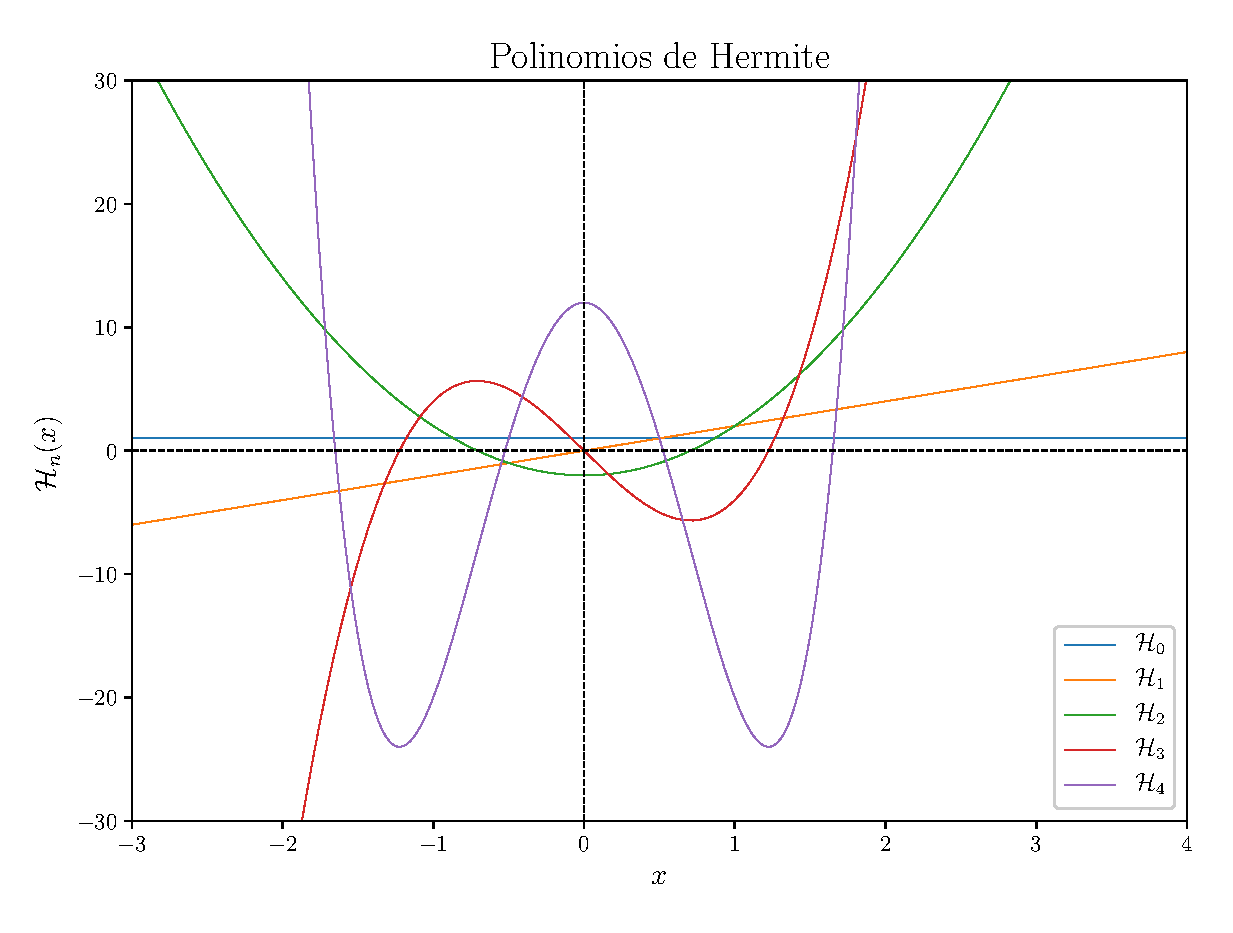
\includegraphics[scale=0.5]{Imagenes/Polinomios_Hermite_01.eps}
%     \caption{Gráfica de los primeros polinomios de Hermite (con pyhton).}
%     \label{figura_003}
% \end{figure}
% \end{frame}
\begin{frame}[plain]
\begin{figure}[H]
    \centering
    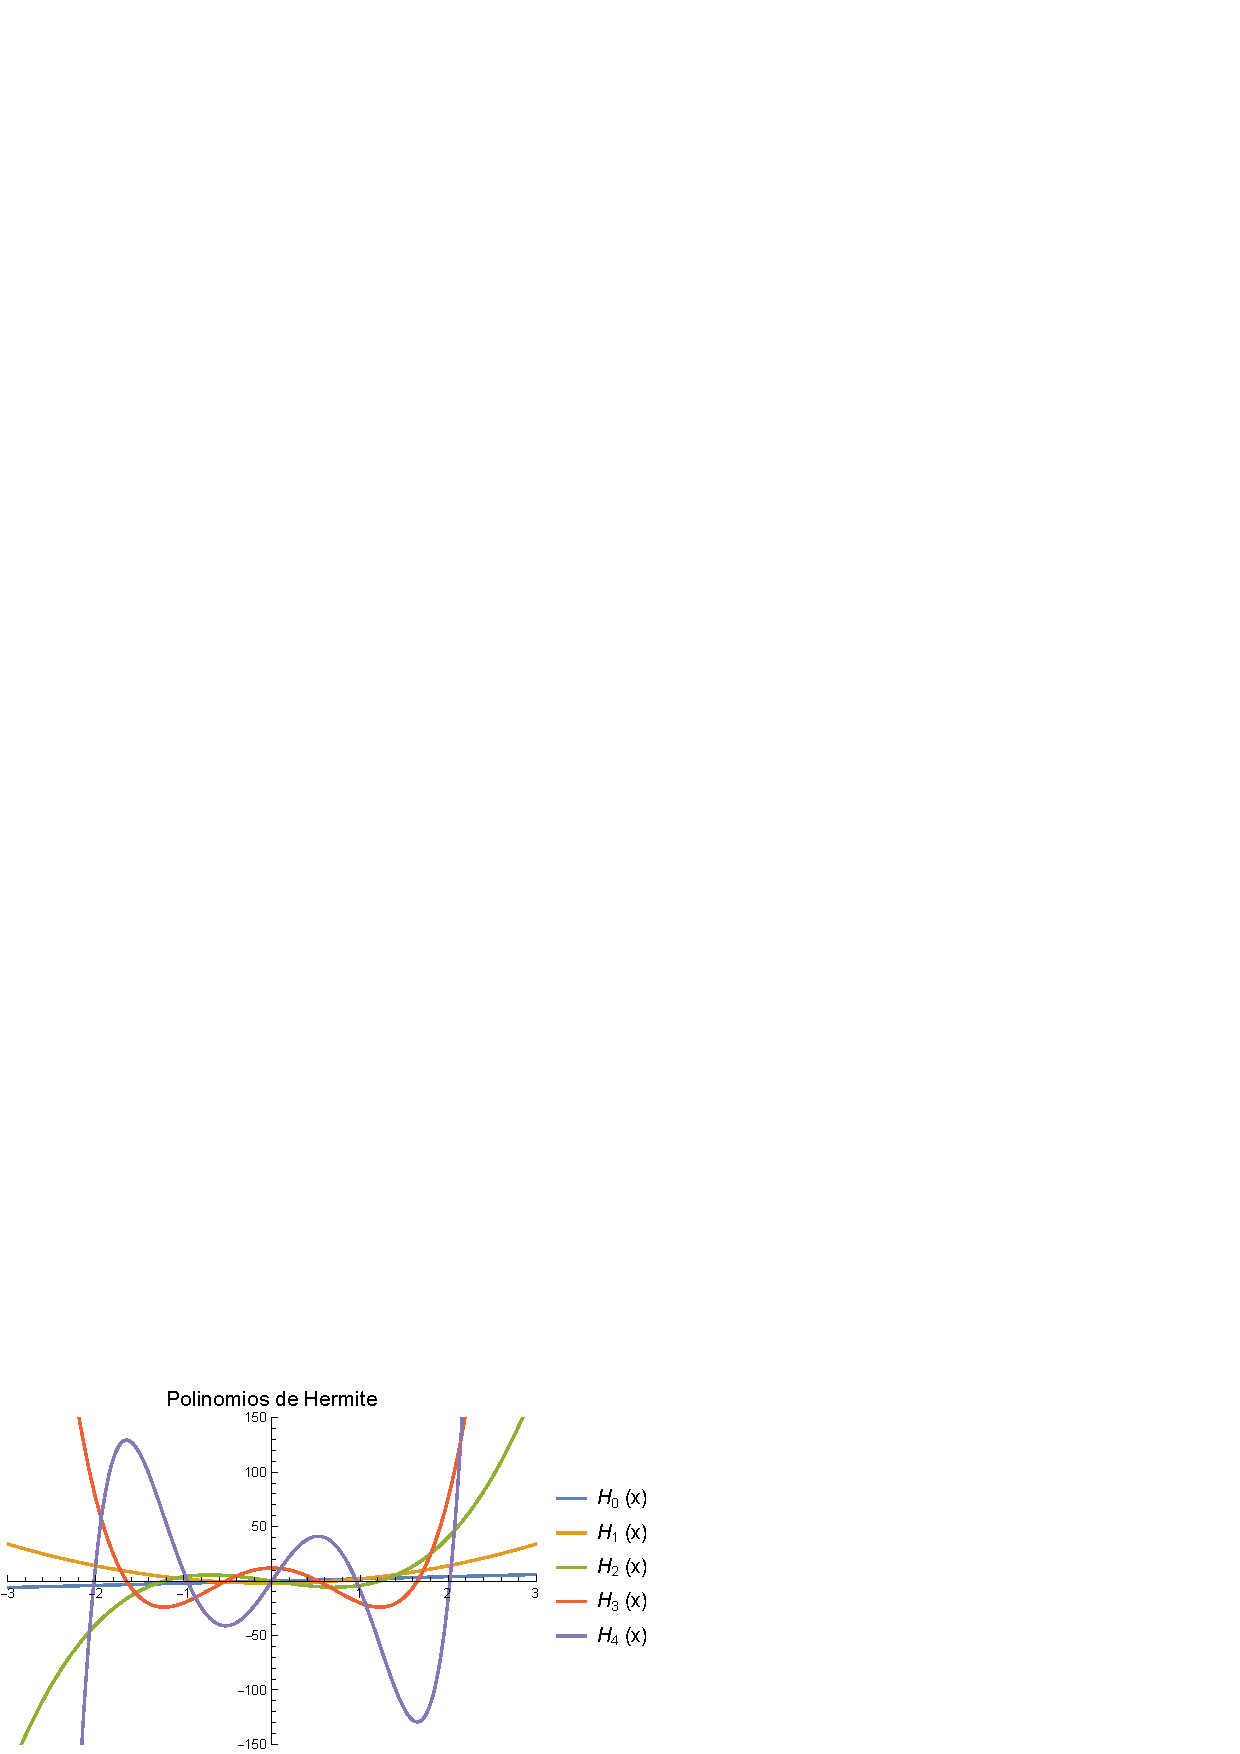
\includegraphics[scale=0.7]{Imagenes/Plot_Hermite_01.pdf}
    \caption{Gráfica de los primeros polinomios de Hermite (con Wolfram).}
    \label{figura_004}
\end{figure}
\end{frame}

\begin{frame}
\frametitle{Convención}
Por tradición, el factor multiplicativo arbitrario se elige de modo que el coeficiente de la potencia más alta de $\xi$ es $2^{n}$.
\end{frame}
\begin{frame}
\frametitle{Convención}
Con esta convención, los estados estacionarios normalizados para el oscilador armónico son:
\pause
\begin{equation}
\psi_{n} (x) = \left( \dfrac{m \, \omega}{\pi \, \hbar} \right)^{1/4} \, \dfrac{1}{\sqrt{2^{n} \, n!}} \, H_{n} (\xi) \, \exp \left( - \dfrac{\xi^{2}}{2} \right)
\label{eq:ecuacion_02_069}
\end{equation}
Son idénticos (por supuesto) a los que obtuvimos algebraicamente en la ec. (\ref{eq:ecuacion_02_050}).
\end{frame}
\begin{frame}
\frametitle{Funciones de onda}
En las siguientes figuras, se han trazado la función $\psi_{n} (x)$ para las primeras $n$'s y su normalización.
\end{frame}
\begin{frame}[plain]
\begin{figure}[H]
    \centering
    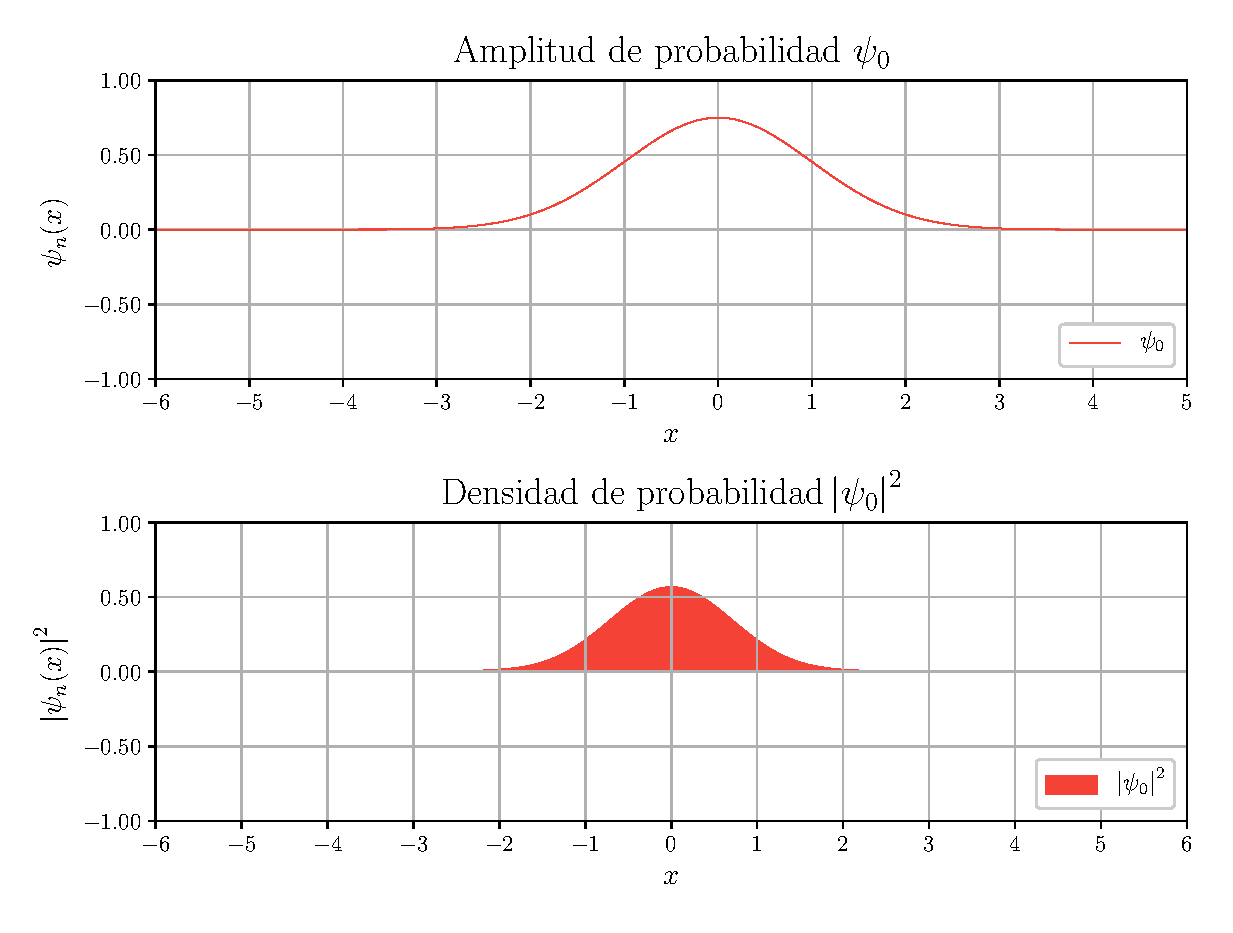
\includegraphics[scale=0.5]{Imagenes/Funcion_Onda_00.eps}
\end{figure}
\end{frame}
\begin{frame}[plain]
\begin{figure}[H]
    \centering
    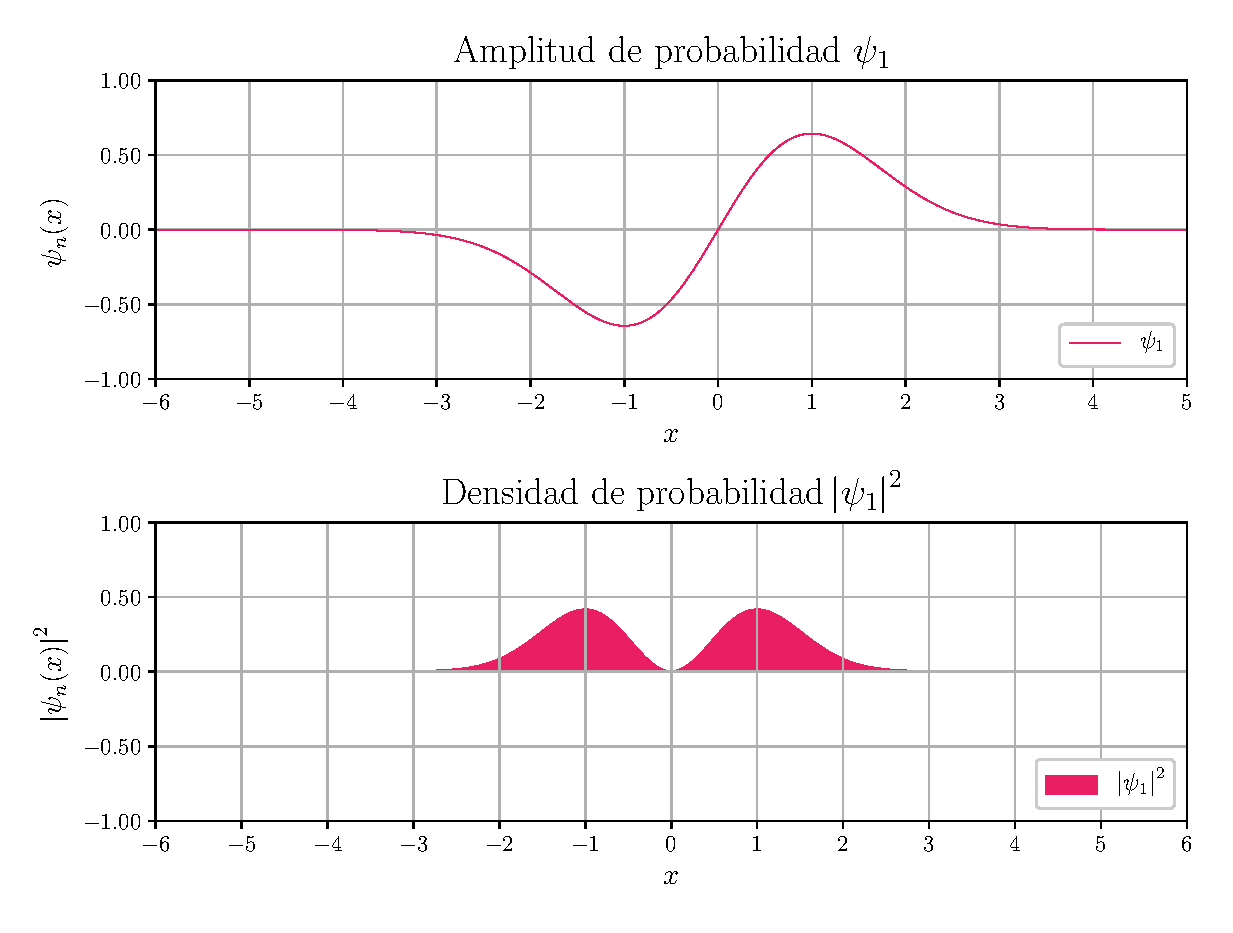
\includegraphics[scale=0.5]{Imagenes/Funcion_Onda_01.eps}
\end{figure}
\end{frame}
\begin{frame}[plain]
\begin{figure}[H]
    \centering
    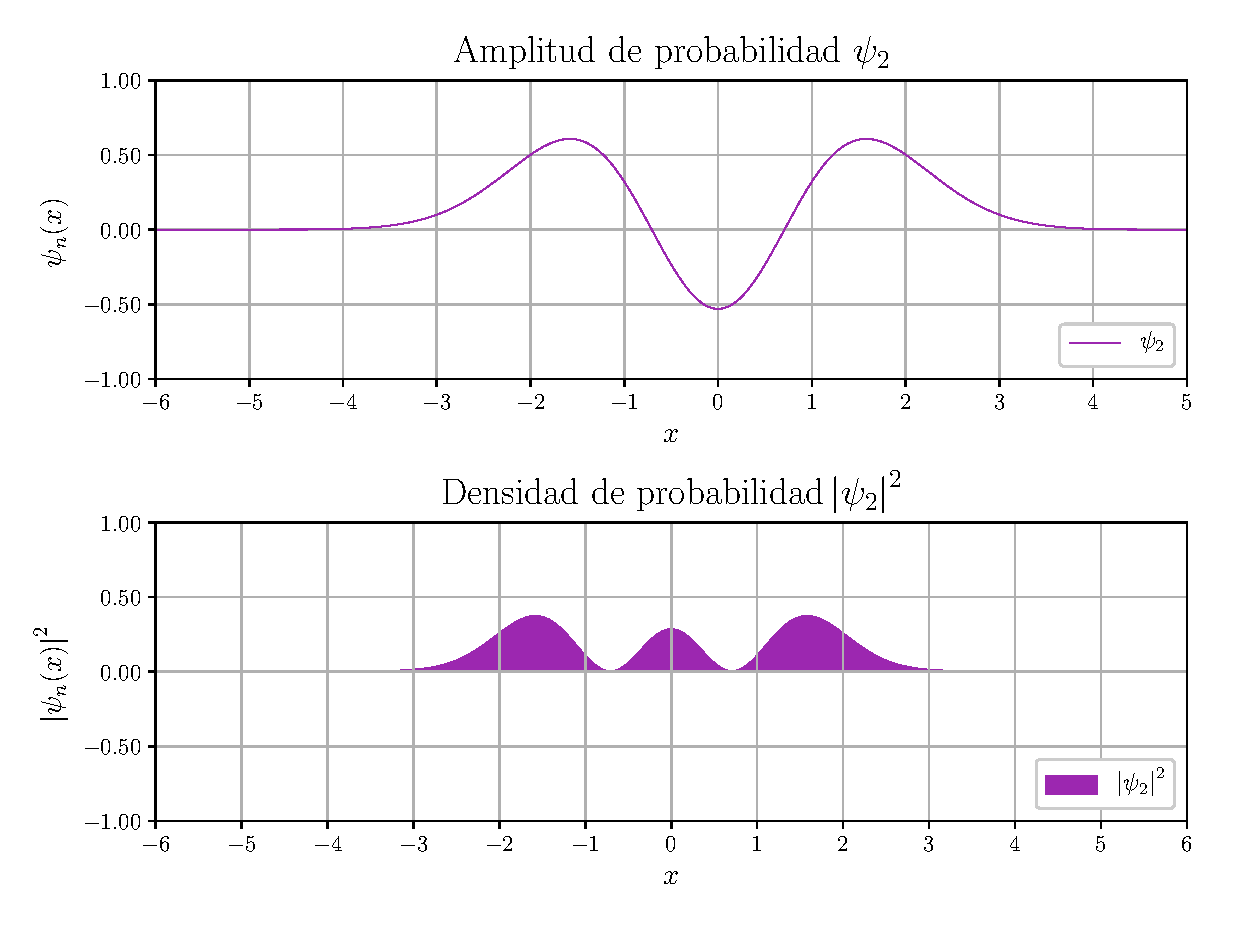
\includegraphics[scale=0.5]{Imagenes/Funcion_Onda_02.eps}
\end{figure}
\end{frame}
\begin{frame}[plain]
\begin{figure}[H]
\centering
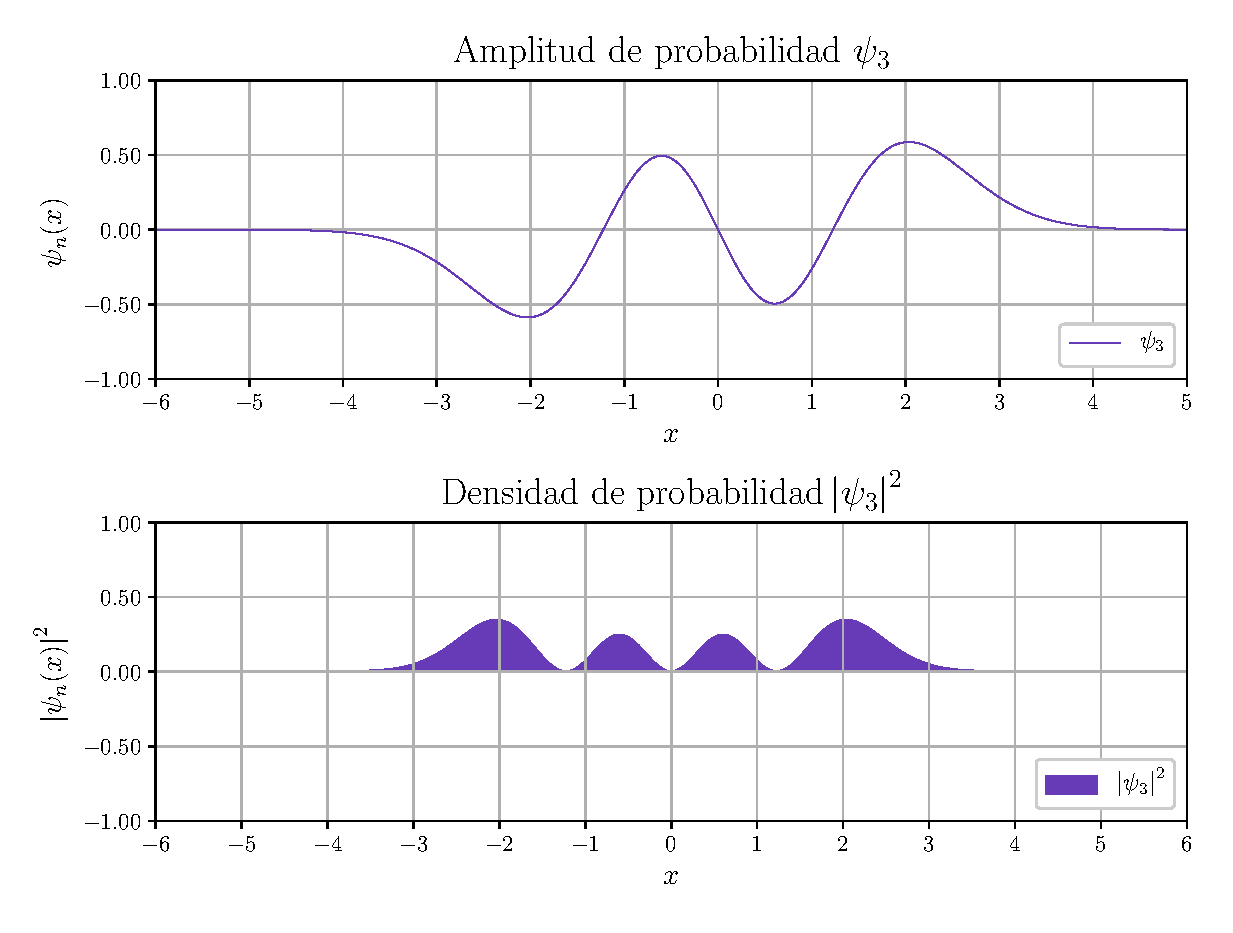
\includegraphics[scale=0.5]{Imagenes/Funcion_Onda_03.eps}
\end{figure}
\end{frame}
\begin{frame}[plain]
\begin{figure}[H]
\centering
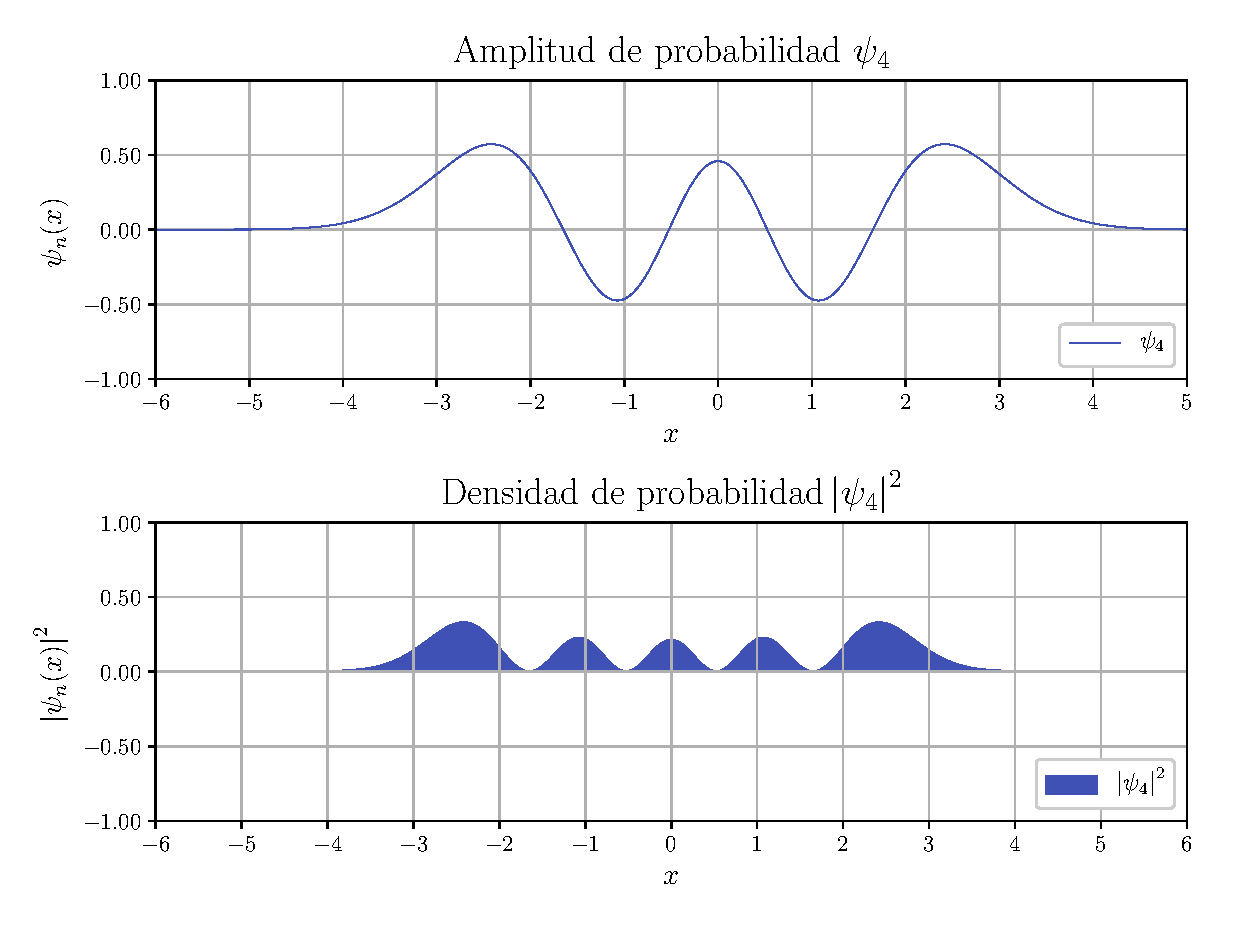
\includegraphics[scale=0.5]{Imagenes/Funcion_Onda_04.eps}
\end{figure}
\end{frame}
\begin{frame}[plain]
\begin{figure}[H]
    \centering
    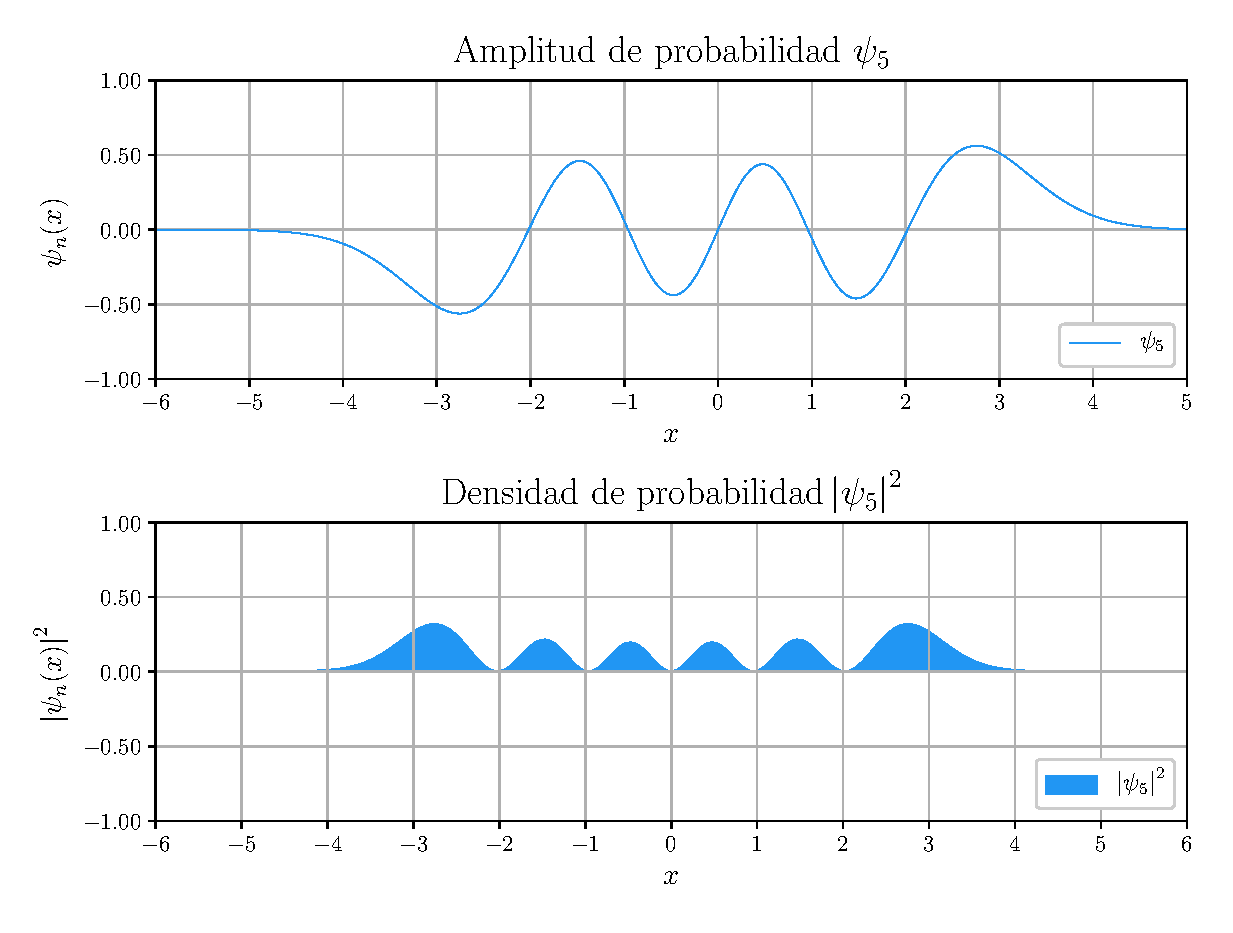
\includegraphics[scale=0.5]{Imagenes/Funcion_Onda_05.eps}
\end{figure}
\end{frame}
\begin{frame}[plain]
\begin{figure}[H]
\centering
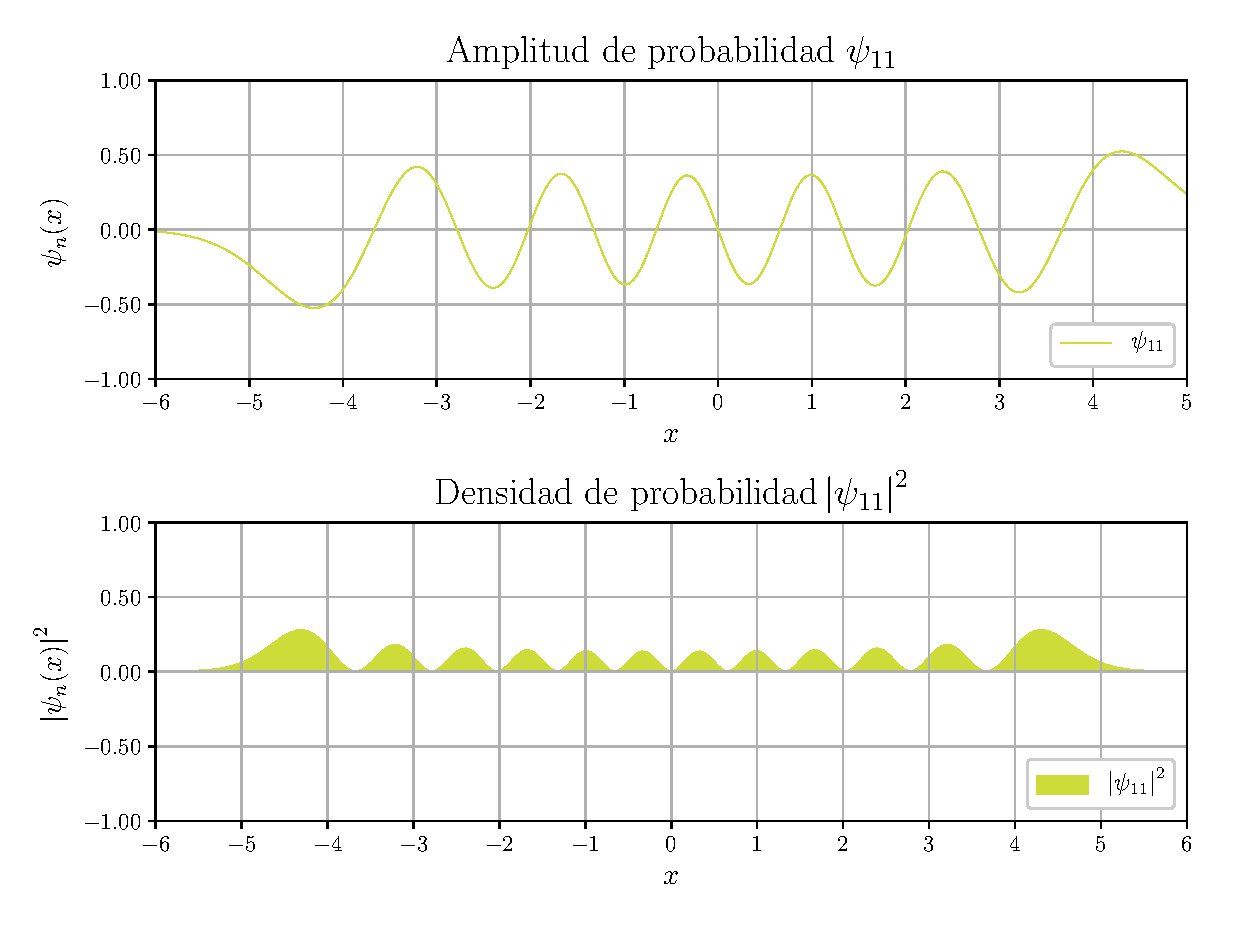
\includegraphics[scale=0.5]{Imagenes/Funcion_Onda_011.eps}
\end{figure}
\end{frame}
\begin{frame}[plain]
\begin{figure}[H]
    \centering
    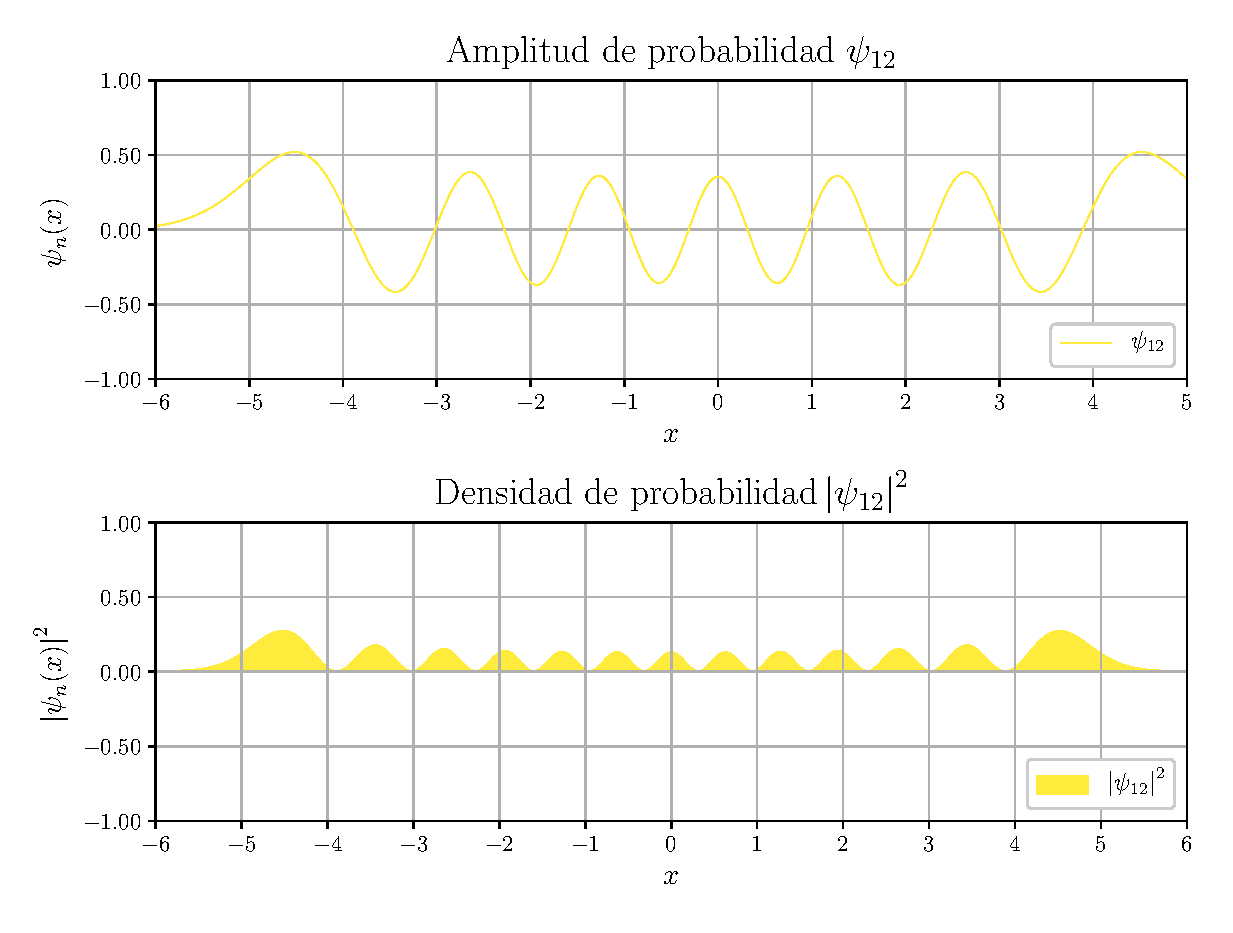
\includegraphics[scale=0.5]{Imagenes/Funcion_Onda_012.eps}
\end{figure}
\end{frame}
\begin{frame}
\frametitle{Comparando el potencial}
En la siguiente gráfica se han superpuesto el potencial parabólico y las funciones de onda normalizadas, esquemáticamente representa la solución a la ecuación de Schrödinger.
\end{frame}
\begin{frame}[plain]
\begin{figure}[H]
    \centering
    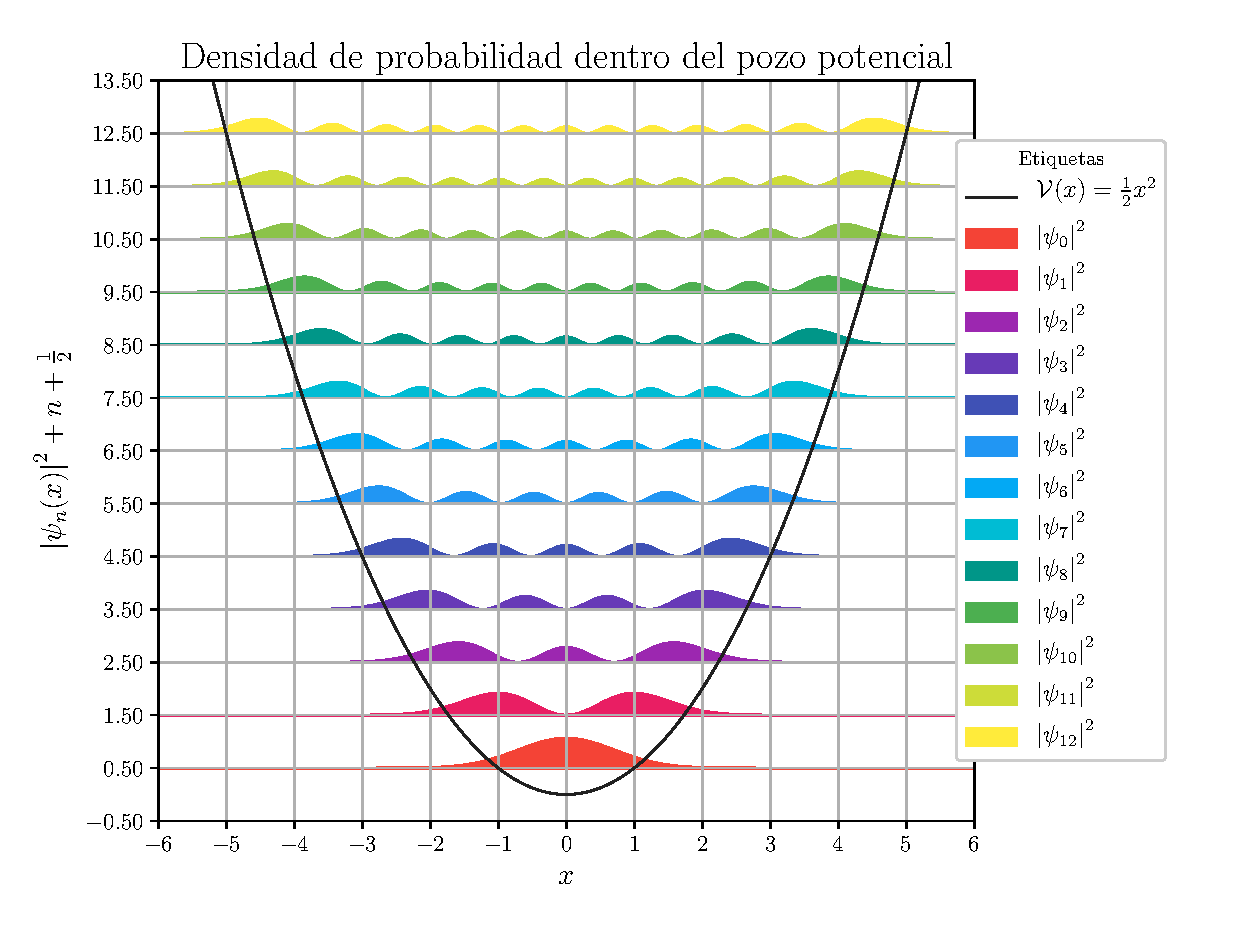
\includegraphics[scale=0.5]{Imagenes/Funciones_Normalizadas_01.eps}
\end{figure}
\end{frame}
\begin{frame}
\frametitle{Propiedades del oscilador}
El oscilador cuántico es sorprendentemente diferente de su contraparte clásica: \pause 
no solo se cuantifican las energías, sino que las distribuciones de posición tienen algunas características extrañas. 
\end{frame}
\begin{frame}
\frametitle{Propiedades del oscilador}
Por ejemplo, la probabilidad de encontrar la partícula fuera del rango permitido clásicamente (es decir, con $x$ mayor que la amplitud clásica para la energía en cuestión) no es cero.
\end{frame}
\begin{frame}
\frametitle{Propiedades del oscilador}
\pause y en todos los estados impares la probabilidad de encontrar la partícula en el centro del pozo de potencial es cero.
\end{frame}
\begin{frame}
\frametitle{Propiedades del oscilador}    
Sólo para valores relativamente grandes de $n$ empezamos a ver alguna semejanza con el caso clásico. 
\end{frame}
\begin{frame}[plain]
\begin{figure}[H]
    \centering
    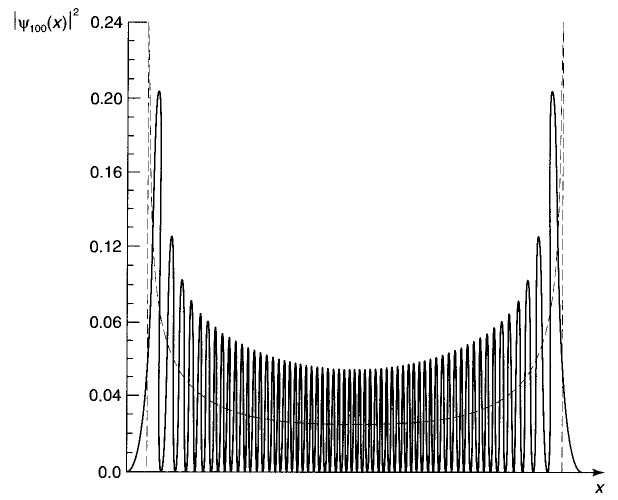
\includegraphics[scale=0.35]{Imagenes/Funcion_Onda_100.png}
    \caption{Gráfica para la función de onda $\abs{\psi_{100}}^{2}$, junto con una distribución clásica (línea punteada).}
    \label{figura_005}
\end{figure}
\end{frame}
\begin{frame}
\frametitle{De la figura}
En la figura (\ref{figura_004}), se han superpuesto la distribución de posición clásica en la cuántica (para $n = 100$).
\end{frame}
\begin{frame}
\frametitle{De la figura}
Si aplanaramos los bultos, los dos encajarían bastante bien, \pause sin embargo, en el caso clásico estamos hablando de la distribución de posiciones en el tiempo para un oscilador.
\end{frame}
\begin{frame}
\frametitle{De la figura}
Mientras que en el caso cuántico estamos hablando de la distribución en un conjunto de sistemas preparados de manera idéntica.
\end{frame}


\section{Propiedades de los Polinomios de Hermite}
\frame[allowframebreaks]{\frametitle{Temas a revisar} \tableofcontents[currentsection, hideothersubsections]}
\subsection{Definición de un valor}

\begin{frame}
\frametitle{Definición}
La normalización de los polinomios ha sido elegida de modo tal que:
\pause
\begin{align*}
H_{0} (x) = 1
\end{align*}
\end{frame}

\subsection{Relaciones de recurrencia}

\begin{frame}
\frametitle{Expresiones}
Algunas de las relaciones de recurrencia de los polinomios de Hermite son:
\pause
\begin{eqnarray*}
\begin{aligned}
H_{n+1} (x) &= 2 \, x \, H_{n} (x) - 2 \, n \, H_{n-1} (x) \\ \pause
\pderivada{H}_{n} (x) &= 2 \, n \, H_{n-1} \\ \pause
H_{n} (x) &= (-)^{n} \, H_{n} (-x) \\ \pause
H_{2n} (0) &= (-)^{n} \, \dfrac{(2 \, n)!}{n!} \\ \pause
H_{2n+1} (0) &= 0
\end{aligned}
\end{eqnarray*}
\end{frame}

\subsection{Fórmula de Rodrigues}

\begin{frame}
\frametitle{La fórmula de Rodrigues}
La fórmula de Rodrigues es una técnica para generar polinomios ortogonales mediante derivadas de una función base. 
\end{frame}
\begin{frame}
\frametitle{La fórmula de Rodrigues}
\begin{align*}
H_{n} (x) &= (-1)^{n} \, e^{x^{2}} \, \dv[n]{n} \left( e^{-x^{2}} \right)
\end{align*}
\end{frame}

\subsection{Función generatriz}

\begin{frame}
\frametitle{La función generatriz}
La normalización de la integral que determina la ortogonalidad de los polinomios $\left\{ H_{n} (x) \right\}$ puede hacerse utilizando la siguiente identidad, \pause que define la función generatriz de los polinomios de Hermite:
\pause
\begin{align*}
\exp \left( -t^{2} + 2 \, x \, t \right) = \nsum_{n=0}^{\infty} \dfrac{H_{n} (x) \, t^{n}}{n!}
\end{align*}
\end{frame}
\begin{frame}
\frametitle{Manejando la expresión}
Se sigue que:
\pause
\begin{align*}
\exp \left( -x^{2} \right) \, & \exp \left( -t^{2} + 2 \, x \, t \right) \, \exp \left( -s^{2} + 2 \, x \, s \right) = \\
&= \nsum_{n=0}^{\infty} \, \nsum_{m=0}^{\infty} \dfrac{e^{-x^{2}}}{n! \, m!} \, t^{n} \, s^{m} \, H_{n} (x) \, H_{m} (x)
\end{align*}
\end{frame}
\begin{frame}
\frametitle{Manejando la expresión}
Integrando con respecto a $x$ en el intervalo $(-\infty, \infty)$ y considerando que:
\pause
\begin{align*}
&\exp \left( -x^{2} \right) \, \exp \left( -t^{2} + 2 x t \right) \, \exp \left( -s^{2} + 2 x s \right) = \\
&= \exp \left( - (x - s - t)^{2} \right) \, \exp \left( 2 s t \right)
\end{align*}
\end{frame}
\begin{frame}
\frametitle{Manejando la expresión}
Con el resultado:
\pause
\begin{align*}
&\scaleint{6ex}_{-\infty}^{\infty} e^{-x^{2}} \, H_{n} (x) \, H_{m} (x) \, \dd{x} = \\[1em]
&= \delta_{m n} \scaleint{6ex}_{-\infty}^{\infty} e^{-x^{2}} \, H_{n}^{2} (x) \, \dd{x}
\end{align*}
\end{frame}
\begin{frame}
\frametitle{Manejando la expresión}
Se obtiene:
\pause
\begin{eqnarray*}
\begin{aligned}
&\nsum_{n=0}^{\infty} \dfrac{(s \, t)^{n}}{(n!)^{2}} \scaleint{6ex}_{-\infty}^{\infty} e^{-x^{2}} \, H_{n}^{2} (x) \, \dd{x} = \sqrt{\pi} \, e^{2 s t } = \\[0.5em] \pause 
&=\sqrt{\pi} \, \nsum_{n=0}^{\infty} \nsum_{n=0}^{\infty} \dfrac{2^{n} \, (s t)^{n}}{n!}
\end{aligned}
\end{eqnarray*}
\end{frame}
\begin{frame}
\frametitle{Manejando la expresión}
De donde:
\pause
\[ \scaleint{6ex}_{-\infty}^{\infty} e^{-x^{2}} \, H_{n}^{2} (x) \, \dd{x} = 2^{n} \, \sqrt{\pi} \, n! \]
\end{frame}

\subsection{Normalización}

\begin{frame}
\frametitle{Normalización de los polinomios}
En consecuencia, la condición de ortogonalidad de los polinomios de Hermite es:
\pause
\begin{eqnarray*}
\begin{aligned}
\scaleint{6ex}_{-\infty}^{\infty} e^{-x^{2}} \, &H_{n} (x) \, H_{m} (x) \dd{x} = 2^{n} \, \sqrt{\pi} \, n! \, \delta_{m n} \\
n = 0, 1, 2, \ldots
\end{aligned}
\end{eqnarray*}
\end{frame}

\subsection{Base completa}

\begin{frame}
\frametitle{Base completa y ortogonal}
El conjunto $\left\{ H_{n }(x) \right\}$ es completo; \pause por tanto cualquier función $f(x)$ definida en el intervalo $(-\infty, \infty)$ puede expandirse en polinomios de Hermite:
\pause
\[ f(x) = \nsum_{n=0}^{\infty} C_{n} \, H_{n} (x) \]
\end{frame}
\begin{frame}
\frametitle{Base completa y ortogonal}
En forma general puede afirmarse que cualquier función definida en $(-\infty, \infty)$ puede expandirse en cualquier base ortogonal definida en $(-\infty, \infty)$.
\end{frame}
\begin{frame}
\frametitle{Base completa y ortogonal}
Expresar la función en una u otra es cambiar de base: la misma función puede expandirse,\pause  por ejemplo, en la base de Hermite $\left\{ H_{n }(x) \right\}$, \pause o en la de Fourier $\left\{ e^{i k x} \right\}$.
\end{frame}

\section{Ejercicios a cuenta}
\frame[allowframebreaks]{\frametitle{Temas a revisar} \tableofcontents[currentsection, hideothersubsections]}
\subsection{Enunciados}

\begin{frame}
\frametitle{Ejercicio 1}
% %Ref. Arfken(2006) 13.1.6 (b)
Demuestra que la expansión de la función \break \hfill $f (x) =x^{2 r + 1}$ en una serie de polinomios de Hermite de orden impar es:
\begin{align*}
x^{2 r +1} &= \dfrac{(2 r + 1)!}{2^{2 r +1}} \nsum_{n=0}^{r} \dfrac{H_{2n+1}(x)}{(2 \, n + 1)! \, (r - n)!} \\[1em]
&{} \hspace{2cm} r = 0, 1, 2, \ldots
\end{align*}
Nota: Considera usar la fórmula de Rodrigues para luego integrar por partes.
\end{frame}
\begin{frame}
\frametitle{Ejercicio 2}
% %Ref. Arfken(2006) 13.1.10
Demuestra que:
\begin{align*}
\scaleint{6ex}_{\bs - \infty}^{\infty} x^{2} \, e^{-x^{2}} \, H_{n}(x) \, H_{n}(x) \dd{x} = \pi^{\frac{1}{2}} \, 2^{n} \, n! \, \bigg( n + \dfrac{1}{2} \bigg)
\end{align*}
Esta integral se presenta en el cálculo del desplazamiento medio cuadrado del oscilador armónico cuántico.
\end{frame}



% \section{La familia de la ecuación de Hermite.}
% A partir de la ecuación de Hermite y utilizando la transformación
% \[ H_{n} (x) = e^{\alpha x^{2}} \, \psi_{n} (\mu), \hspace{2cm} \mu = x^{b} \]
% se obtiene la primera familia de Hermite
% \begin{align*}
% &{} b^{2} \, \dv[2]{\psi_{n} (\mu)}{\mu} \, \mu^{2 (b-1)/b} + \dv{\psi_{n}(\mu)}{\mu} \left[ b \, (b-1) \mu^{\frac{b-2}{2}}  + \right. \\
% &+\left. 2 \, b \, (2 \, a - 1) \, \mu \right] + \left[ 4 \, a \, (a - 1) \, \mu^{2/b} + 2 \, n + 2 \, a \right] \, \psi_{n} (\mu) = 0
% \end{align*}
% cuya solución es
% \[ \psi_{n} (\mu) = e^{-\alpha x^{2}} \, H_{n} (x) = \exp \left( - \dfrac{a x^{2}}{b} \right) \, H_{n} (\mu^{1/b}) \]
% \begin{enumerate}[label=\roman*.)]
% \item Con $a = 0, b = 1$, se recupera la ecuación de Hermite.
% \item Si $b = 1, a = 1/2$, se obtiene la ecuación de \textbf{Weber-Hermite}:
% \begin{equation}
% \dv[2]{\psi_{n} (x)}{x} + [ 1 + 2 \, n - x^{2} ] \, \psi_{n} (x) = 0
% \label{eq:ecuacion_08_65}
% \end{equation}
% \end{enumerate}
% Con $\mu = x$ y $\psi_{n} (x) = e^{-x^{2}/2} / H_{n} (x)$. Esta última describe el oscilador armónicos unidimensional en mecánica cuántica. Nótese que la base $\left\{ \psi_{n} (x) \right\}$ es ortonormal.
% %Referencia: Luis de la Peña. Introducción a la mecánica cuántica. Cap. 11
% % \section{Introducción.}
% % Pasaremos ahora a estudiar con detenimiento uno de los sistemas físicos de
% % mayor interés teórico, \textbf{el oscilador armónico cuántico}. Para simplificar el tratamiento
% % nos restringimos al caso unidimensional, que carece de degeneración (el
% % oscilador armónico en más de una dimensión es un problema degenerado que,
% % para su tratamiento cabal, requiere en la teoría clásica de la teoría del momento
% % angular.
% % \par
% % El oscilador armónico ocurre en el caso cuántico de manera similar a como se da clásicamente:
% % \emph{aparece cuando potenciales más o menos complicados se aproximan en la región
% % de un mínimo con curvas parabólicas}. Por lo tanto, se trata esencialmente de la
% % teoría de oscilaciones poco energéticas en torno a un mínimo de potencial, situación
% % que se da con frecuencia con átomos, moléculas, etc. Además, el empleo frecuente
% % del análisis de Fourier para estudiar sistemas complejos en términos de osciladores
% % elementales hace del oscilador armónico uno de los problemas más importantes de
% % la física teórica, sin considerar su interés metodológico debido al hecho de poseer
% % solución exacta.
% % \par
% % En esta sección nuestro interés primordial se centra en el estudio de la dinámica
% % del sistema. El problema que vamos a abordar ahora (la solución de la ecuación
% % completa de Schrödinger) es más complicado que el de determinar los eigenestados
% % y el espectro del oscilador armónico cuántico, pero preferimos iniciar el estudio del
% % oscilador mostrando que se trata en efecto de osciladores, exhibiendo y analizando
% % las oscilaciones. Con esto, tendremos oportunidad de ver en qué son similares y
% % en qué se distinguen los osciladores clásicos de los cuánticos. Con esta idea en
% % mente, iniciamos el tema con el estudio de un paquete de osciladores armónicos,
% % posponiendo un poco el de los estados propios del oscilador. Por otro lado sucede
% % que, de todos los posibles paquetes de osciladores, hay algunos muy particulares
% % cuyo comportamiento es el más simple. Puesto que nos interesa —por claridad—
% % mantener la máxima simplicidad posible, nos limitaremos al estudio de estos últimos,
% % que son los paquetes (gaussianos) de mínima dispersión y máxima coherencia, como
% % tendremos oportunidad de comprobar.
% % El potencial de un oscilador armónico cuántico unidimensional está dado por la
% % expresión usual
% % %Referencia: Graton. Introducción a la mecánica cuántica. Cap. 9
% % \begin{equation}
% % V(x) = \dfrac{1}{2} \, m  \, \omega^{2} \, x^{2}
% % \label{eq:ecuacion_09_068}
% % \end{equation}
% % donde $\omega$ es la frecuencia clásica del oscilador y $m$ la masa. La forma de la ec. (\ref{eq:ecuacion_09_068}) del potencial $V (x)$ es de gran importancia práctica, pues es una aproximación para cualquier energía potencial arbitraria en el entorno de un punto de equilibrio estable. 
% % \par
% % El oscilador armónico simple es también importante porque el comportamiento de sistemas tales como las vibraciones de un medio elástico y del campo electromagnético en una cavidad se pueden describir como la superposición de un número infinito de osciladores armónicos simples. Al cuantificar esos sistemas nos encontramos entonces con la mecánica cuántica de muchos osciladores armónicos lineales de diferentes frecuencias. Por tal motivo, todas las teorías de campos modernas utilizan los resultados que vamos a obtener.
% % \par
% % El Hamiltoniano del oscilador armónico simple es
% % \begin{equation}
% % H = \dfrac{p^{2}}{2 m} + \dfrac{1}{2} \, m \, \omega^{2} \, x^{2}
% % \label{eq:ecuacion_09_069}
% % \end{equation}
% % por lo que la ecuación de Schrödinger independiente del tiempo es:
% % \begin{equation}
% % - \dfrac{h^{2}}{2 m} \dv[2]{\psi}{x} + \dfrac{1}{2} m \, \omega^{2} \, x^{2} \, \psi = E \, \psi
% % \label{eq:ecuacion_09_070}
% % \end{equation}
% % Para un manejo más sencillo de las expresiones, sustituimos las variables $x \to \xi$ y $p \to \eta$, definidos por
% % \begin{align}
% % \begin{aligned}
% % x &= \xi \, \sqrt{\dfrac{\hbar}{m \omega}} \\[1em]
% % p &= \eta \, \sqrt{m \, \hbar \, \omega}
% % \end{aligned}
% % \label{eq:ecuacion_07_071}
% % \end{align}
% % Se puede comprobar fácilmente que $\xi$ y $\eta = - i \dv*{\xi}$ cumplen la relación de conmutación
% % \begin{equation}
% % [\xi, \eta] = \xi \, \eta - \eta \, \xi = i
% % \label{eq:ecuacion_09_072}
% % \end{equation}
% % En términos de  $\xi$ y $\eta$, el Hamiltoniano se escribe
% % \begin{equation}
% % H =  \hbar \, \omega \mathcal{H} \hspace{1.5cm} \mathcal{H} = \dfrac{1}{2} (\eta^{2} + \xi^{2})
% % \label{eq:ecuacion_09_073}
% % \end{equation} 
% % entonces la ec. (\ref{eq:ecuacion_09_070}) toma la forma
% % \begin{equation}
% % \dv[2]{\psi}{\xi} + (2 \, \varepsilon - \xi^{2}) \, \psi = 0 \hspace{1.5cm} E = \hbar \, \omega \, \varepsilon
% % \label{eq:ecuacion_09_074}
% % \end{equation}
% % Veamos el comportamiento de $\psi (\xi)$ cuando $\xi \to \pm \infty$. Para valores finitos de $\varepsilon$, es fácil verificar que
% % \begin{equation}
% % \psi (\xi \to \pm \infty) \rightarrow \exp(-\xi^{2}/2)
% % \label{eq:ecuacion_09_075}
% % \end{equation}
% % de manera que $\psi$ tiene el comportamiento de una gaussiana.
% % \par
% % Es inmediato verificar por sustitución directa que
% % \begin{equation}
% % \psi_{0} (\xi) = \exp(-\xi^{2}/2)
% % \label{eq:ecuacion_09_076}
% % \end{equation}
% % es una soluci{on de la ec. (\ref{eq:ecuacion_09_074}) y corresponde al valor propio $\varepsilon = 1/2$. En efecto, si $\varepsilon = 1/2$, se cumplen
% % \begin{equation}
% % \dv[2]{\psi_{0}}{\xi} + (2 \, \varepsilon - \xi^{2}) \, \psi_{0} = - \psi_{0} + \xi^{2} \, \psi_{0} + (2 \, \varepsilon - \xi^{2}) \, \psi_{0} = 0
% % \label{eq:ecuacion_09_077}
% % \end{equation}
% % Para encontrar las demás funciones propias y valores propios, vamos a usar una sencilla y elegante técnica de operadores, que es diferente de los métodos que se emplean habitualmente en los textos elementales de Mecánica Cuántica. Hacemos así porque esta técnica es el prototipo de otras semejantes que se aplican en una variedad de problemas.
% % \par
% % El método se funda en las propiedades de conmutación de ciertos operadores no Hermitianos oportunamente definidos, y permite encontrar sistemáticamente mediante un procedimiento recursivo todas las funciones propias y sus correspondientes valores propios a partir de $\psi_{0}$ y de $\varepsilon$. Para eso definimos el operador
% % \begin{equation}
% % a = \dfrac{1}{\sqrt{2}} (\xi + i \, \eta) = \dfrac{1}{\sqrt{2}} \left( \xi + \dv{\xi} \right)
% % \label{eq:ecuacion_09_078}
% % \end{equation}
% % que no es Hermitiano, y su adjunto es
% % \begin{equation}
% % a^{\dagger} = \dfrac{1}{\sqrt{2}} (\xi - i \, \eta) = \dfrac{1}{\sqrt{2}} \left( \xi - \dv{\xi} \right)
% % \label{eq:ecuacion_09_079}
% % \end{equation}
% % En términos de $a$ y $a^{\dagger}$, el operador $\mathcal{H}$ se expresa como
% % \begin{equation}
% % \mathcal{H} = a^{\dagger} \, a + \dfrac{1}{2}
% % \label{eq:ecuacion_09_080}
% % \end{equation}
% % El conmutador $[a, a^{\dagger}]$ es
% % \begin{equation}
% % [a, a^{\dagger}] = a \, a^{\dagger} - a^{\dagger} \, a = 1
% % \label{eq:ecuacion_09_081}
% % \end{equation}
% % Puesto que $\mathcal{H}$ y $a^{\dagger} \, a$ conmutan, las funciones propias de $\mathcal{H}$ y $a^{\dagger} \, a$ son las mismas, de modo que para encontrar los estados estacionarios es suficiente resolver el problema de valores propios de $a^{\dagger} \, a$. Si llamamos $\lambda_{n}\, (n = 0, 1, 2, \ldots)$ a los valores propios y $\psi_{n}$ las correspondientes funciones propias, la ecuación que queremos resolver es
% % \begin{equation}
% % a^{\dagger} \, a \, \psi_{n} = \lambda_{n} \, \psi_{n}
% % \label{eq:ecuacion_09_082}
% % \end{equation}
% % Primero veremos que los valores propios no pueden ser negativos. De la ec. (\ref{eq:ecuacion_09_082}) se tiene que
% % \begin{equation}
% % (\psi_{n}, a^{\dagger} \, a \, \psi_{n}) = ( a \, \psi_{n}, a \, \psi_{n} ) = \lambda_{n} (\psi_{n}, \psi_{n})
% % \label{eq:ecuacion_09_083}
% % \end{equation}
% % donde usamos la definición de operador adjunto. Puesto que la norma de una función no puede
% % ser negativa, concluimos que
% % \begin{equation}
% % \lambda_{n} \geq 0
% % \label{eq:ecuacion_09_084}
% % \end{equation}
% % Si $\psi_{k}$ es una función propia de $a^{\dagger} \, a$, entonces $a^{\dagger} \, \psi_{k}$ es también una función propia; en efecto usando la relación de conmutación (\ref{eq:ecuacion_09_081}), vemos que:
% % \begin{equation}
% % (a^{\dagger} \, a) \, a^{\dagger} \, \psi_{k} = a^{\dagger} (a^{\dagger} \, a + 1) \, \psi_{k} = (\lambda_{k} + 1) \, a^{\dagger} \, \psi_{k}
% % \label{eq:ecuacion_09_085}
% % \end{equation}
% % Por lo tanto $a^{\dagger} \, \psi_{k}$ es una función propia con valor propio $\lambda_{k} + 1$. Del mismo modo se obtiene
% % \begin{equation}
% % (a^{\dagger} \, a) \, a \, \psi_{k} = a (a^{\dagger} \, a + 1) \, \psi_{k} = (\lambda_{k} + 1) \, a \, \psi_{k}
% % \label{eq:ecuacion_09_086}
% % \end{equation}
% % que muestra que $a \, \psi_{k}$ es una autofunción de $a^{\dagger} \, a$ con autovalor $\lambda_{k} - 1$ . Debido a estas propiedades $a^{\dagger}$ y $a$ se denominan \emph{operador de subida y operador de bajada}, respectivamente.
% % \par
% % Operando reiteradamente con $a^{\dagger}$ y $a$ sobre una función propia $\psi_{k}$ dada, podemos generar nuevas funciones propias correspondientes a diferentes valores propios, del mismo modo como se suben o se bajan los peldaños de una escalera.
% % \par
% % Sin embargo, la condición (\ref{eq:ecuacion_09_084}) limita la cantidad de veces que se
% % puede aplicar el operador de bajada, porque cuando se llega un valor propio $0 leq \lambda_{0} < 1$, la aplicación del operador de bajada no permite ya encontrar una nueva función propia, pues sería una función propia correspondiente a un valor propio que viola la condición (\ref{eq:ecuacion_09_084}). Por lo tanto para el peldaño más bajo de la escalera $(n = 0)$ se debe cumplir
% % \begin{equation}
% % a^{\dagger} \, a \, \psi_{0} = \lambda_{0} \, \psi_{0}, \hspace{1.5cm} 0 \leq \lambda_{0} < 1
% % \label{eq:ecuacion_09_087}
% % \end{equation}
% % y también
% % \begin{equation}
% % a \, \psi_{0} = 0
% % \label{eq:ecuacion_09_088}
% % \end{equation}
% % y por consiguiente, el menor valor propio de $a^{\dagger} \, a$ es
% % \begin{equation}
% % \lambda_{0} = 0
% % \label{eq:ecuacion_09_089}
% % \end{equation}
% % Partiendo entonces de $\psi_{0}$ y de $\lambda_{0} = 0$ podemos obtener todas las demás funciones propias y valores propios por aplicación reiterada del operador de subida $a^{\dagger}$. Pero nosotros ya conocemos $\psi_{0}$, que está dado por la ec. (\ref{eq:ecuacion_09_076}):
% % \begin{equation}
% % \psi_{0} (\xi) = \exp(- \xi^{2}/2) 
% % \label{eq:ecuacion_09_090}
% % \end{equation}
% % Por consiguiente la $n-$ésima función propia, y su correspondiente valor propio son
% % \begin{equation}
% % \psi_{n} \propto \left( a^{\dagger} \right)^{n} \, \psi_{0} (\xi) = \left[ \dfrac{1}{\sqrt{2}} \left( \xi - \dv{\xi} \right) \right]^{n} \, \exp(-\xi^{2}/2), \hspace{1cm} \lambda_{n} = n
% % \label{eq:ecuacion_09_091}
% % \end{equation}
% % Usando las ecs. (\ref{eq:ecuacion_09_074}) y (\ref{eq:ecuacion_09_080}), obtenemos que
% % \begin{equation}
% % H \, \psi_{n} = \hbar \, \omega (n + \dfrac{1}{2}) \, \psi_{n}
% % \label{eq:ecuacion_09_092}
% % \end{equation}
% % por lo que los valores propios de la energía son
% % \begin{equation}
% % E_{n} = \hbar \, \omega (n + \dfrac{1}{2}) \hspace{1cm} n = 0, 1, 2, \ldots
% % \label{eq:ecuacion_09_093}
% % \end{equation}
% % Observamos que a diferencia del caso clásico, la energía del oscilador \emph{no es nula} en el estado fundamental $(n = 0)$ sino que todavía vale $\hbar \omega / 2$ . Este resultado de la teoría de Schrödinger difiere del que se obtuvo en la Teoría Cuántica Antigua a partir de los postulados de cuantificación Planck y de Wilson-Sommerfeld. La energía $\hbar \omega / 2$ se denomina energía de punto cero del oscilador armónico y su existencia es un fenómeno cuántico que se puede entender en base al principio de incertidumbre.

% %Referencia:: Sepúlveda - Lecciones de Física Matemática Cap. 8.5 Polinomios de Hermite.
% % \section{Funciones de Hermite.}
% % La ecuación de Hermite, tiene una aplicación en física, quizá la más importante que es la del oscilador armónico en mecánica cuántica, tiene la forma:
% % \begin{equation}
% % \ddot{H}(x) - 2 \, x \,  \dot{H}(x) + 2\, n \, H(x) = 0
% % \label{eq:ecuacion_08_58}
% % \end{equation}
% % La forma autoadjunta para una ED sabemos que es de la forma
% % \[ \dv{x} \left[ q(x) \, \dv{H(x)}{x} \right] + r(x) \, H(x) + \lambda \, p(x) \, H(x) = 0 \]
% % por lo que para la ec. de Hermite, resulta ser
% % \begin{equation}
% % \dv{x} \left[ \exp(-x^{2}) \, \dv{H(x)}{x} \right] + 2 \, n \, \exp(-x^{2}) \, H(x) = 0
% % \label{eq:ecuacion_08_59}
% % \end{equation}
% % La solución a esta ecuación forma una base ortogonal con factor de peso $p(x) = \exp(-x^{2})$, en el intervalo $(-\infty, \infty)$, ya que en dicho intervalo
% % \[ [q \, W]\eval_{-\infty}^{\infty} = [ \exp(-x^{2}) \, W ]\eval_{-\infty}^{\infty} = 0 \]
% % La ortogonalidad queda expresada por
% % \[ \scaleint{6ex}_{-\infty}^{\infty} \exp(-x^{2}) \, H_{n}(x) \, H_{m}(y) \, \dd{x} = 0, \hspace{1cm} \mbox{ si } n \neq m \]
% % Con lo que vemos que la ortogonalidad de las funciones propias está asociada a la elección particular del dominio de la variable independiente.
% % \par
% % Aplicamos el método de Frobenius para encontrar una solución:
% % \begin{align*}
% % H(x) &= \nsum_{\alpha = 0}^{\infty} a_{\alpha} \, x^{\alpha+k} \\[1em]
% % \dot{H}(x) &= \nsum_{\alpha = 0}^{\infty} a_{\alpha} \, (\alpha + k) \, x^{\alpha+k-1} \\[1em]
% % \ddot{H}(x) &= \nsum_{\alpha = 0}^{\infty} a_{\alpha} \, (\alpha + k) \, (\alpha + k - 1) \, x^{\alpha+k-2}
% % \end{align*}
% % re-emplazando en la ecuación (\ref{eq:ecuacion_08_58}) y factorizando los términos
% % \[ \nsum_{\alpha = 0}^{\infty} a_{\alpha} \, (\alpha + k) \, (\alpha + k - 1) \, x^{\alpha+k-2} - \nsum_{\alpha=0}^{\infty} a_{\alpha} \, [ 2 \, (\alpha + k) - 2 \, n] \, x^{\alpha+k} = 0 \]
% % que puede escribirse como
% % \[ \nsum_{\alpha=-2}^{\infty} a_{\alpha + 2} \, ( \alpha + k + 2) \, (\alpha + k + 1)\, x^{\alpha+k} - \nsum_{\alpha=0}^{\infty} a_{\alpha} \, [2 \, (\alpha + k) - 2 \, n] \, x^{\alpha+k} = 0 \]
% % escribiendo los dos primeros términos de la serie
% % \begin{align*}
% %  a_{0}(k) \, (k - 1)\, x^{k-2} &+ a_{1} \, (k + 1)(k)^{\alpha-1} + \\
% % &+ \nsum_{\alpha=0}^{\infty} \left\{ a_{\alpha + 2} \, (\alpha + k +2) \, (\alpha + k + 1) + \right. \\
% % &- \left. a_{0} \, [2 (\alpha + k ) - 2 \, n] \right\} \, x^{\alpha+k} = 0 
% % \end{align*}
% % donde reconocemos las ecuaciones de índices:
% % \begin{align*}
% % a_{0}\, k \, (k-1) &= 0 \\
% % a_{1} \, k\, (k+1) &= 0 \\
% % a_{\alpha+2}\, (\alpha + k + 2) \, (\alpha + k + 1) - a_{\alpha} \, [2 \, (\alpha + k) - 2 \, n] &= 0, \hspace{1cm} \alpha=0, 1, 2, \ldots
% % \end{align*}
% % Revisamos que:
% % \begin{enumerate}
% % \item De la primera expresión: si $a_{0} \neq 0$, entonces $k=0$ ó $k=1$.
% % \item De la segunda expresión: con $k=0$ se sigue que $a_{1} \neq 0$ y de $k=1$, se concluye que $a_{1} = 0$.
% % \item De la tercera ecuación de índices con $k=0$, se obtiene
% % \[ a_{\alpha+2} = \dfrac{2a_{\alpha}(\alpha - n)}{(\alpha + 2)(\alpha + 1)} \hspace{1cm} \alpha = 0, 1, 2, \ldots \]
% % \end{enumerate}
% % Explícitamente los primeros coeficientes son
% % \begin{align*}
% % a_{2} &= \dfrac{(-) \, 2 \, n}{2!} \, a_{0} \\
% % a_{3} &= \dfrac{(-) \, 2 \, (n-1)}{3!} \, a_{1} \\
% % a_{4} &= \dfrac{(-) \, 2 \, a_{2} \, (2 - n)}{4 \times 3} = \dfrac{2^{2} \, (-)^{2} \, (n) \, (n - 2)}{4!} a_{0} \\
% % \vdots
% % \end{align*}
% % Entonces tenemos
% % \begin{align*}
% % H(x) &= a_{0} \, \left[ 1 + \dfrac{(-) 2 \, n}{2!}\, x^{2} + \dfrac{(-) \, 2^{2} \, n \, (n - 2)}{4!}\, x^{4} + \right. \\
% % &+ \left. \dfrac{(-)^{3} \, 2^{3} \, n \, (n-2)(n-4) }{6!}\, x^{6} + \ldots \right] + \\
% % &+ a_{1} \, \left[ x + \dfrac{(-) \, 2 \, (n-1)}{3!} \, x^{3} + \dfrac{(-)^{2} \, 2^{2} \, (n-1)(n-3)}{5!}\, x^{5} + \right.\\
% % &+ \left. \dfrac{(-)^{3} \, 2^{3} \, (n-1)(n-3)(n-5)}{7!} \, x^{7} + \ldots \right]
% % \end{align*}
% % Ambas series son divergentes en $x \to \pm \infty$. Si se incluyen estos dos extremos y se quiere lograr convergencia es necesario cortar las series y convertirlas en polinomios.
% % \par
% % La serie en $a_{0}$ requiere que $n$ = par positivo y la serie en $a_{1}$ requiere $n$ = impar positivo. Puesto que $n$ no puede ser simultáneamente par e impar en las series para $a_{0}$ y $a_{1}$, si $n$ = par, la segunda serie es divergente y si $n$ = impar la primera diverge.
% % \par
% % Las series convergentes serán las de nuestro interés, y conformarán los \emph{Polinomios de Hermite}.
% % \\
% % Puede demostrarse que con $n \neq$ entero, $H(x) \propto x^{2} \, \exp(x^{2})$ para $x \to \pm \infty$, lo que muestra la no convergencia para $n$ no entero.
% % \par
% % Consideremos $n$ = par. La serie para $a_{0}$, con $n=2\, m, \; m = 0, 1, 2, \ldots$ será
% % \begin{align*}
% % H(x) &= a_{0} \, \left[ 1 + \dfrac{(-) \, 2^{2} \, m}{2!} \, x^{2} + \dfrac{(-)^{2} \, 2^{4} \, m \, (m - 1)}{4!} \, x^{4} + \right. \\
% % &+ \left. \dfrac{(-)^{3} \, 2^{6} \, m \, (m-1)(m-2)}{6!} \, x^{6} + \ldots \right] \\[1em]
% % H(x) &= a_{0}\, \left[ 1 + \dfrac{(-)\, 2^{2}\, m}{2!} \, x^{2} + \ldots + \dfrac{(-)^{3} \, 2^{6}\, m!}{(m-3)! \, 6!} \, x^{6} + \ldots \right. \\[0.5em]
% % &+ \left. \dfrac{(-)^{p} \, (2 \, x)^{2\, p}\, m!}{(m-p)! \, (2\, p)!} + \ldots \right] \\[0.5em]
% % &= m!\, a_{0} \, \nsum_{p=0}^{\infty} \dfrac{(-)^{p}\, (2\, x)^{2\, p}}{(m-p)! \, (2\, p)!}
% % \end{align*}
% % Se definen los polinomios de Hermite de orden par, en la forma
% % \begin{equation}
% % H_{2\, m} (x) = (-)^{m} \, (2\, m)! \nsum_{p=0}^{\infty} \dfrac{(-)^{p} \, (2\, x)^{2\, p}}{(m-p)!\, (2p)!}
% % \label{eq:ecuacion_08_60}
% % \end{equation}
% % Revisemos que efectivaente la ecuación (\ref{eq:ecuacion_08_60}) es un polinomio, ya que para $p > m : 1 / (m-p)! \to 0$. Esto significa que la suma se extiende entre $0$ y $m$.
% % \par
% % De manera análoga, para $n=$ impar, con $n = 2 \, m + 1, \hspace{0.5cm} m=0, 1, 2, \ldots$
% % \begin{align*}
% % H(x) & = a_{1} \, \left[ x + \dfrac{(-) \, 2^{2} \, m}{3!} \, x^{2} + \dfrac{(-)^{2} \, 2^{4} \, m \, (m - 1)}{5!} \, x^{5} + \right. \\
% % & + \left. \dfrac{(-)^{3} \, 2^{6} \, m \, (m-1)(m-2)}{7!} \, x^{7} + \ldots \right] \\[1em]
% % H(x) & = a_{1}\, \left[ x + \dfrac{(-)\, 2^{2}\, m}{3!} \, x^{3} + \ldots + \dfrac{(-)^{3} \, 2^{6}\, m!}{(m-3)! \, 7!} \, x^{7} + \ldots + \right. \\[0.5em]
% % &+  \left. \dfrac{(-)^{p} \, 2^{2 \, p} \, m!}{(m-p)! \, (2\, p + 1)!} \, x^{2p+1} + \ldots \right] \\[0.5em]
% % & = a_{1} \, m! \nsum_{p=0}^{\infty} \dfrac{(-)^{p}\, (2\, x)^{2\, p+1}}{(m-p)! \, (2\, p + 1)!}  
% % \end{align*}
% % Definimos los polinomios de Hermite de orden impar como:
% % \begin{equation}
% % H_{2m+1} (x) = (-)^{m} \, (2 \, m + 1)! \, \nsum_{p=0}^{\infty} \dfrac{(-)^{p} \, (2 \, x)^{2p+1}}{(m-p)! \, (2 \, p + 1)!}
% % \label{eq:ecuacion_08_61}
% % \end{equation}
% % donde la suma da términos diferentes de cero sólo entre $0$ y $m$. En forma compacta se tiene la expresión:
% % \begin{equation}
% % \boxed{H_{n}(x) = n! \, \nsum_{p=0}^{N} \dfrac{(-)^{p}}{(n - 2 \, p)! \, p!} \, (2 \, x)^{n-2p}}
% % \label{eq:ecuacion_08_62}
% % \end{equation}
% % con $N=n/2$ si $n$ es par, o $N=n-1/2$ si $n$ es impar.
% % \par
% % La primera ecuación de índices provee para el exponente $k$ en la serie de Frobenius un segundo valor: $k = 1$. Es directo comprobar que nada nuevo se añade al desarrollo anterior.
% % \par
% % Los primeros polinomios de Hermite son:
% % \begin{align*}
% % H_{0}(x) &= 1 \\
% % H_{1}(x) &= 2 \, x \\
% % H_{2}(x) &= 4 \, x^{2} - 2 \\
% % H_{3}(x) &= 8 \, x^{3} - 12 \, x \\
% % H_{4}(x) &= 16 \, x^{4} - 48 \, x^{2} + 12 \\
% % H_{5}(x) &= 32 \, x^{5} - 160 \, x^{3} + 120 \, x
% % \end{align*}
% % La normalización de los polinomios ha sifo elegida de modo tal que $H_{0}(x) = 1$.
% % \par
% % Algunas de las propiedades de los polinomios de Hermite son:
% % \begin{align*}
% % H_{n} (x) &= (-)^{n} \, e^{x^{2}} \, \dv[n]{n} \left( e^{-x^{2}} \right) \\
% % H_{n+1} (x) &= 2 \, x \, H_{n} (x) - 2 \, n \, H_{n-1} (x) \\
% % \dot{H}_{n} (x) &= 2 \, n \, H_{n-1} \\
% % H_{n} (x) &= (-)^{n} \, H_{n} (-x) \\
% % H_{2n} (0) &= (-)^{n} \, \dfrac{(2 \, n)!}{n!} \\
% % H_{2n+1} (0) &= 0
% % \end{align*}
% % La primera de estas se conoce como fórmula de Rodrigues.
% % \par
% % La normalización de la integral de ortogonalidad de los polinomios $\left\{ H_{n} (x) \right\}$ puede hacerse utilizando la siguiente identidad, que define la función generatriz de los polinomios de Hermite:
% % \[ \exp \left( -t^{2} + 2 \, x \, t \right) = \nsum_{n=0}^{\infty} \dfrac{H_{n} (x) \, t^{n}}{n!} \]
% % se sigue que:
% % \begin{align*}
% % \exp \left( -x^{2} \right) \, & \exp \left( -t^{2} + 2 \, x \, t \right) \, \exp \left( -s^{2} + 2 \, x \, s \right) = \\
% % &= \nsum_{n=0}^{\infty} \, \nsum_{m=0}^{\infty} \dfrac{e^{-x^{2}}}{n! \, m!} \, t^{n} \, s^{m} \, H_{n} (x) \, H_{m} (x)
% % \end{align*}
% % Integrando con respecto a $x$ en el intervalo $(-\infty, \infty)$ y considerando que
% % \[ \exp \left( -x^{2} \right) \, \exp \left( -t^{2} + 2 x t \right) \, \exp \left( -s^{2} + 2 x s \right) = \exp \left( - (x - s - t)^{2} \right) \, \exp \left( 2 s t \right) \]
% % y con el resultado
% % \[ \scaleint{6ex}_{-\infty}^{\infty} e^{-x^{2}} \, H_{n} (x) \, H_{m} (x) \, \dd x = \delta_{m n} \scaleint{6ex}_{-\infty}^{\infty} e^{-x^{2}} \, H_{n}^{2} (x) \, \dd x \]
% % se obtiene:
% % \[ \nsum_{n=0}^{\infty} \dfrac{(s t)^{n}}{(n!)^{2}} \scaleint{6ex}_{-\infty}^{\infty} e^{-x^{2}} \, H_{n}^{2} (x) \, \dd x = \sqrt{\pi} \, e^{2 s t } = \sqrt{\pi} \, \nsum_{n=0}^{\infty} \nsum_{n=0}^{\infty} \dfrac{2^{n} \, (s t)^{n}}{n!} \]
% % de donde:
% % \[ \scaleint{6ex}_{-\infty}^{\infty} e^{-x^{2}} \, H_{n}^{2} (x) \, \dd x = 2^{n} \, \sqrt{\pi} \, n! \]
% % En consecuencia, la condición de ortogonalidad es:
% % \begin{equation}
% % \boxed{ \scaleint{6ex}_{-\infty}^{\infty} e^{-x^{2}} \, H_{n} (x) \, H_{m} (x) \dd x = 2^{n} \, \sqrt{\pi} \, n! \, \delta_{m n} \hspace{1cm} n = 0, 1, 2, \ldots }
% % \end{equation}
% % El conjunto $\left\{ H_{n }(x) \right\}$ es completo; por tanto cualquier función $f(x)$ definida en el intervalo $(-\infty, \infty)$ puede expandirse en polinomios de Hermite:
% % \[ f(x) = \nsum_{n=0}^{\infty} C_{n} \, H_{n} (x) \]
% % En forma general puede afirmarse que cualquier función definida en $(-\infty, \infty)$ puede expandirse en cualquier base ortogonal definida en $(-\infty, \infty)$.
% % \par
% % Expresar la función en una u otra es cambiar de base: la misma función puede expandirse, por ejemplo, en la base de Hermite $\left\{ H_{n }(x) \right\}$, o en la de Fourier $\left\{ e^{i k x} \right\}$.
% % \section{La familia de la ecuación de Hermite.}
% % A partir de la ecuación de Hermite y utilizando la transformación
% % \[ H_{n} (x) = e^{\alpha x^{2}} \, \psi_{n} (\mu), \hspace{2cm} \mu = x^{b} \]
% % se obtiene la primera familia de Hermite
% % \begin{align*}
% % &{} b^{2} \, \dv[2]{\psi_{n} (\mu)}{\mu} \, \mu^{2 (b-1)/b} + \dv{\psi_{n}(\mu)}{\mu} \left[ b \, (b-1) \mu^{\frac{b-2}{2}}  + \right. \\
% % &+\left. 2 \, b \, (2 \, a - 1) \, \mu \right] + \left[ 4 \, a \, (a - 1) \, \mu^{2/b} + 2 \, n + 2 \, a \right] \, \psi_{n} (\mu) = 0
% % \end{align*}
% % cuya solución es
% % \[ \psi_{n} (\mu) = e^{-\alpha x^{2}} \, H_{n} (x) = \exp \left( - \dfrac{a x^{2}}{b} \right) \, H_{n} (\mu^{1/b}) \]
% % \begin{enumerate}[label=\roman*.)]
% % \item Con $a = 0, b = 1$, se recupera la ecuación de Hermite.
% % \item Si $b = 1, a = 1/2$, se obtiene la ecuación de \textbf{Weber-Hermite}:
% % \begin{equation}
% % \dv[2]{\psi_{n} (x)}{x} + [ 1 + 2 \, n - x^{2} ] \, \psi_{n} (x) = 0
% % \label{eq:ecuacion_08_65}
% % \end{equation}
% % \end{enumerate}
% % Con $\mu = x$ y $\psi_{n} (x) = e^{-x^{2}/2} / H_{n} (x)$. Esta última describe el oscilador armónicos unidimensional en mecánica cuántica. Nótese que la base $\left\{ \psi_{n} (x) \right\}$ es ortonormal.
% % \section{El oscilador armónico cuántico.}
% % Como una aplicación importante de los polinomios de Hermite consideremos la cuantización de la energía del oscilador armónico.
% % \par
% % De acuerdo con la mecánica cuántica, un oscilador armónico unidimensional, cuya energía potencial es $V = \frac{1}{2} k \, x^{2}$ puede describirse mediante la ecuación de Schrödinger:
% % \[ - \dfrac{\hbar^{2}}{2 \, m} \, \dv[2]{\psi (x)}{x} + V (x) \, \psi (x) =  E \, \psi (x) \]
% % donde $\psi (x)$ representa la función de onda, $\hbar$ es la constante de Planck dividida entre $2 \, \pi$, $m$ es la masa del oscilador y $E$ su energía total. 
% % \par
% % Cambiando a la nueva variable adimensional: $y = x/\alpha$, donde $\alpha$ tendrá la misma dimensión que $x$, y utilizando $\omega^{2} = k/m$, siendo $\omega$ la frecuencia angular del oscilador y $k$ la constante del resorte, podremos escribir:
% % \[ \dv[2]{\psi}{y} - \left( \dfrac{\omega \, m \, \alpha^{2}}{\hbar}  \right)^{2} \, y^{2} \, \psi  + \left( \dfrac{2 \, m \, E \, \alpha^{2}}{\hbar^{2}} \right) \, \psi = 0 \] 
% % La adimensionalidad de $y$ y la homogeneidad en $\psi$ de la ecuación permiten escoger un valor para $\alpha$, tal que el primer paréntesis tenga el valor de $1$, esto es:
% % \[ \dfrac{\omega \, m \, \alpha}{\hbar} = 1 \hspace{1.5cm} \mbox{de donde } \alpha^{2} = \dfrac{\hbar}{m \, \omega} \]
% % El segundo paréntesis (adimensional), lo llamaremos $\lambda$:
% % \[ \lambda = \dfrac{2 \, m \, E \, \alpha^{2}}{\hbar} = \dfrac{2 \, E}{\hbar \, \omega} \]
% % Por lo que la ecuación del oscilador toma la forma:
% % \begin{equation}
% % \dv[2]{\psi}{y} + (\lambda - y^{2}) \, \psi = 0
% % \label{eq:ecuacion_08_66}
% % \end{equation}
% % Esta expresión, conocida como \emph{ecuación de Weber-Hermite}, corresponde, a la primera familia de Hermite con $b = 1$ y $a = 1/2$, tal que su solución es la función de Weber-Hermite de orden $n$ entero:
% % \begin{equation}
% % \psi_{n} (y) = e^{y^{2}/2} \, H_{n} (y)
% % \label{eq:ecuacion_08_67}
% % \end{equation}
% % y por tanto $1 + 2 \, n = \lambda$
% % \par
% % Dado que $\lambda = 2 \, E / \hbar \, \omega$, se tiene que
% % \begin{align}
% % \dfrac{2 \, E}{\hbar \, \omega} &= 1 + 2 \, n \nonumber \\
% % E &= \left(n + \dfrac{1}{2} \right) \, \hbar \, \omega. \hspace{1.5cm} n \geq 0
% % \label{eq:ecuacion_08_68}
% % \end{align}
% % Como $n$ toma valores enteros, se sigue que la energía del oscilador está cuantizada y que hay una energía mínima o de punto cero: $E_{min} = \hbar \, \omega /2$.
% % \par
% % La secuencia de niveles de energía (\ref{eq:ecuacion_08_68}) tiene el espaciamiento $\Delta E = \hbar \, \omega$ postulado por Planck en 1900. Lo notable es que hay un mínimo en la energía que no aparece en la teoría de Planck y que es exigido por el principio de incertidumbre: \emph{un oscilador armónico no puede estar en reposo}. Si lo estuviera, sería en $x = 0$ que es el punto de equilibrio; en consecuencia podríamos conocer simultáneamente su posición y velocidad, lo que no es compatible con el principio de incertidumbre de Heisenberg.
% % \par
% % La función de onda normalizada del oscilador será entonces, de acuerdo con la ec. (\ref{eq:ecuacion_08_67}):
% % \begin{align}
% % \psi_{n} (y) = \dfrac{1}{(2^{2} \, \sqrt{\pi} \, n!)^{1/2}} \, e^{-y^{2}/2} \, H_{n} (y) \hspace{1.5cm} y = \dfrac{x}{\alpha} = x \, \sqrt{\dfrac{m \, \omega}{\hbar}}
% % \label{eq:ecuacion_08_69}
% % \end{align}
% % Explícitamente, los primeros niveles de energía tienen la forma:
% % \begin{align*}
% % \psi_{0} (y) &= e^{-y^{2}/2} \hspace{2.6cm} E = \hbar \, \omega /2 \\
% % \psi_{1} (y) &= 2 \, x \, e^{-y^{2}/2} \hspace{2cm} E = 3 \, \hbar \, \omega /2 \\
% % \psi_{2} (y) &= (4 \, y^{2} - 2) \, e^{-y^{2}/2} \hspace{0.7cm} E = 5 \, \hbar \, \omega /2 \\
% % \end{align*}
% % \section{Operadores escalera.}
% % Una de las identidades que satisface la función de Hermite es:
% % \begin{equation}
% % H_{n-1} (x) = \dfrac{1}{2 \, n} \, \dv{x} H_{n} (x)
% % \label{eq:ecuacion_08_70}
% % \end{equation}
% % Según esta expresión, dado un $H_{n} (x)$ todos los anteriores pueden ser deducidos de él. Otra de las identidades es
% % \[ H_{n+1} (x) = 2 \, x \, H_{n} (x) - 2 \, n \, H_{n-1} (x) \]
% % Si de estas dos ecuaciones se elimina $H_{n-1} (x)$, se obtiene
% % \begin{equation}
% % H_{n+1} (x) = \left( 2 \, x - \dv{x} \right) \, H_{n} (x)
% % \label{eq:ecuacion_08_71}
% % \end{equation}
% % expresión que nos dice: dado un $H_{n} (x)$ todos los que le siguen pueden deducirse de él. Basta entonces con un $Hn(x)$ para generar los demás. Los operadores 
% % \[ \dfrac{1}{2 \, n} \dv{x} \hspace{2cm} 2 \, x - \dv{x} \]
% % son los operadores escalera de los polinomios de Hermite.
% % \par
% % En lo que sigue introduciremos los operadores escalera asociados a las funciones de onda del oscilador armónico cuántico dadas por la ecuación (\ref{eq:ecuacion_08_69}). Reemplazando $H_{n} (y)$ de la ecuación (\ref{eq:ecuacion_08_69}) en las ecuaciones (\ref{eq:ecuacion_08_70}) y (\ref{eq:ecuacion_08_71}) obtenemos:
% % \begin{align*}
% % \sqrt{2 \, n} \, \psi_{n-1} (y) &= \left( y + \dv{x} \right) \, \psi_{n} (y) \\
% % \sqrt{2 \, (n + 1)} \, \psi_{n+1} (y) &= \left( y - \dv{x} \right) \, \psi_{n} (y)
% % \end{align*}
% % que pueden ser escritos como:
% % \begin{align}
% % \begin{aligned}
% % \hat{a} \, \psi_{n} &= \sqrt{n} \, \psi_{n-1} \\
% % \hat{a}^{\dagger} \, \psi_{n} &= \sqrt{n+1} \, \psi_{n+1}
% % \end{aligned}
% % \label{eq:ecuacion_08_72}
% % \end{align}
% % donde los operadores $\hat{a}$ y $\hat{a}^{\dagger}$ están definidos por las ecuaciones
% % \[ \hat{a} = \dfrac{1}{\sqrt{2}} \, \left( y + \dv{y} \right) \hspace{1.5cm} \hat{a}^{\dagger} = \dfrac{1}{\sqrt{2}} \, \left( y - \dv{y} \right) \]
% % Estos operadores bajan y suben, respectivamente, estados cuánticos del oscilador. De la primera ecuación con $n = 0$ se obtiene la función de onda normalizada del estado base:
% % \[ \psi_{0} (y) = \pi^{-1/4} \, e^{-y^{2}/2} \]
% % A partir de ésta, pueden calcularse todas las funciones de onda del oscilador armónico mediante la expresión:
% % \begin{equation}
% % \psi_{n} = \dfrac{1}{\sqrt{n!}} \, \left( a^{\dagger} \right)^{n} \, \psi_{0}
% % \label{eq:ecuacion_08_73}
% % \end{equation}

\end{document}